\documentclass[11pt,a4paper]{article}

% ---------- Packages ----------
\usepackage[utf8]{inputenc}
\usepackage[T1]{fontenc}
\usepackage[english]{babel}
\usepackage[margin=2.5cm, top=2cm]{geometry} % slightly smaller top margin
\usepackage{graphicx}
\usepackage{booktabs}
\usepackage{tabularx}
\usepackage{float}
\usepackage{placeins} % provides \FloatBarrier
\usepackage{caption}
\usepackage{subcaption}
\usepackage{amsmath,amssymb}
\usepackage{xcolor}
\usepackage{enumitem}
\usepackage{parskip} % no paragraph indent, small space between paragraphs
\usepackage[hidelinks]{hyperref}
\usepackage{cleveref}
\crefname{figure}{Figure}{Figures} % "Figure 2" instead of "fig. 2"
\crefname{table}{Table}{Tables}
\crefname{section}{Section}{Sections}
\crefname{subsection}{Section}{Sections}
\usepackage[nottoc]{tocbibind} % adds References to the table of contents
\usepackage[titles]{tocloft}    % finer control of the table of contents
\setlength{\cftbeforesecskip}{0.5em} % less space above each section entry, so the contents fit on one page
\usepackage{tikz}
\usetikzlibrary{calc,patterns,arrows.meta}

% ---------- Colours ----------
\definecolor{primary}{RGB}{20,20,20}   % near-black (headings)
\definecolor{accent}{HTML}{1F77B4}    % blue
\definecolor{tpgreen}{RGB}{16,64,44}   % title page: dark green
\definecolor{tpaccent}{RGB}{70,160,100} % title page: green

% Figure palette: muted colours (same as seaborn's "deep" palette, sns.set_palette("deep"))
\definecolor{cblue}{HTML}{4C72B0}
\definecolor{corange}{HTML}{DD8452}
\definecolor{cgreen}{HTML}{55A868}
\definecolor{cred}{HTML}{C44E52}
\definecolor{cpurple}{HTML}{8172B3}
\definecolor{cbrown}{HTML}{937860}
\definecolor{ccyan}{HTML}{64B5CD}

% All section, subsection and subsubsection headings in near-black
\usepackage{sectsty}
\allsectionsfont{\color{primary}}

% Placeholder for unfinished text (remove before submission)
\newcommand{\todo}[1]{\textcolor{red}{\textbf{TODO:} #1}}

% Indicative page targets from the task description.
% Switch to \showtargetsfalse before submission to hide them all.
\newif\ifshowtargets
\showtargetstrue
\newcommand{\pagetarget}[1]{%
  \ifshowtargets
    \noindent{\small\itshape\textcolor{gray}{Target length: #1 pages (indicative)}}\par\medskip
  \fi}

\begin{document}

% ---------- Title page ----------
% Faded lattice transmission tower, drawn with TikZ: \pylon{x}{y}{height}
\tikzset{declare function={
  hw(\y) = ifthenelse(\y<=0.62, 0.22-0.15*\y/0.62, 0.07-0.025*(\y-0.62)/0.30); % half-width of the tower body
}}
\newcommand{\pylon}[3]{%
  \begin{scope}[shift={(#1,#2)}, scale=#3]
    % main legs, waist and peak
    \draw (-0.22,0) -- (-0.07,0.62) -- (-0.045,0.92) -- (0,1.0) -- (0.045,0.92) -- (0.07,0.62) -- (0.22,0);
    % footings
    \foreach \s in {-1,1} \draw (\s*0.25,0) -- (\s*0.19,0);
    % lattice panels of the body (X-bracing and horizontal members)
    \foreach \ya/\yb in {0/0.10, 0.10/0.20, 0.20/0.30, 0.30/0.39, 0.39/0.48, 0.48/0.56, 0.56/0.62,
                         0.62/0.69, 0.69/0.76, 0.76/0.82, 0.82/0.87, 0.87/0.92}{
      \draw ({-hw(\ya)},\ya) -- ({hw(\yb)},\yb);
      \draw ({hw(\ya)},\ya) -- ({-hw(\yb)},\yb);
      \draw ({-hw(\yb)},\yb) -- ({hw(\yb)},\yb);
    }
    % cross arms as triangular trusses (lower arm at 0.62, upper arm at 0.82)
    \foreach \s in {-1,1}{
      % lower arm
      \draw (\s*0.07,0.62) -- (\s*0.42,0.62) -- (\s*0.07,0.685);
      \foreach \xa/\xb in {0.07/0.1575, 0.1575/0.245, 0.245/0.3325, 0.3325/0.42}{
        \draw (\s*\xa,0.62) -- (\s*\xb,{0.685-0.065*(\xb-0.07)/0.35});
        \draw (\s*\xb,0.62) -- (\s*\xb,{0.685-0.065*(\xb-0.07)/0.35});
      }
      % upper arm
      \draw (\s*0.053,0.82) -- (\s*0.30,0.82) -- (\s*0.053,0.87);
      \foreach \xa/\xb in {0.053/0.115, 0.115/0.177, 0.177/0.238, 0.238/0.30}{
        \draw (\s*\xa,0.82) -- (\s*\xb,{0.87-0.05*(\xb-0.053)/0.247});
        \draw (\s*\xb,0.82) -- (\s*\xb,{0.87-0.05*(\xb-0.053)/0.247});
      }
      % insulator strings with discs
      \foreach \xi/\yi in {0.40/0.62, 0.28/0.82}{
        \draw (\s*\xi,\yi) -- (\s*\xi,\yi-0.065);
        \foreach \k in {1,...,5}
          \draw (\s*\xi-0.012,{\yi-0.011*\k}) -- (\s*\xi+0.012,{\yi-0.011*\k});
      }
    }
    % earth-wire peak
    \draw (-0.035,1.0) -- (0.035,1.0);
  \end{scope}}

\newgeometry{left=4.5cm,right=2cm,top=2.5cm,bottom=2.5cm} % shifted right, clear of the band
\begin{titlepage}

\begin{tikzpicture}[remember picture,overlay]
  % Wide band along the left edge, shaded from dark to lighter green
  \shade[left color=tpgreen, right color=tpgreen!75!tpaccent]
    (current page.north west) rectangle ([xshift=2.6cm]current page.south west);
  % Double accent stripe
  \fill[tpaccent] ([xshift=2.75cm]current page.north west) rectangle ([xshift=2.95cm]current page.south west);
  \fill[tpaccent!50] ([xshift=3.05cm]current page.north west) rectangle ([xshift=3.1cm]current page.south west);

\end{tikzpicture}

\centering
\vspace*{\fill}

{\color{tpaccent}\large\scshape TDT4259 -- Group Project\par}
\vspace{1.5em}
{\color{tpgreen}\rule{0.6\textwidth}{1.2pt}\par}
\vspace{1.5em}
{\color{tpgreen}\huge\bfseries Day-Ahead Hourly\\[0.3em]
 Electricity Consumption Forecasting\par}
\vspace{0.8em}
{\Large\color{tpgreen} for a Nordic Electricity Retailer\par}
\vspace{0.5em}
{\large\itshape Aneo case\par}
\vspace{1.5em}
{\color{tpgreen}\rule{0.6\textwidth}{1.2pt}\par}

\vspace{3em}
{\large
Nils Henrik Hoelfeldt Lund \\[0.3em]
Jørgen August Bolseth \\[0.3em]
Thomas Myrseth \\[0.3em]
Niklas Unneland \\[0.3em]
Camilla Eriksen \\[0.3em]
Truls Elverum \par}

\vspace{3em}
{\large Norwegian University of Science and Technology (NTNU)\\[0.3em]
October 2026\par}

\vspace*{\fill}
\vspace{4cm} % keep the text above the power lines
\end{titlepage}
\restoregeometry

% ---------- Front matter ----------
\pagenumbering{roman}

% ---------- Abstract ----------
\begin{abstract}
\noindent
A Nordic electricity retailer must nominate its expected consumption for each hour of the next day, and deviations between forecast and actual consumption are settled as imbalances at prices that can differ substantially from the spot price. We forecast the retailer's hourly consumption for six price areas (NO1--NO5 and FI), issued at 10:00 for the next day, when metered consumption is only available up to five days earlier. The forecast therefore uses consumption lags of at least six days, the temperature forecast for the target day and calendar information.
We follow the chain from problem to monitoring. Models are compared with a same-hour-last-week baseline on a chronological hold-out period, with features checked for data leakage, and the forecast quality is translated into the retailer's imbalance in MWh. \todo{On the test period the best model reduces MAE from 0.49\,MW to 0.31\,MW (about 38\,\%) compared with the baseline; check against final results and add imbalance reduction.}
We also design and test a protocol for missing inputs at forecast time. In simulated outages it keeps the error close to that of complete data when some consumption lags are missing, and limits it to 0.89\,MW when all consumption features are missing, compared with 2.79\,MW for the baseline.
The models are deliberately simple and explainable rather than state of the art. We state where the evidence is thin: only one year of data, a test period of winter and early spring, no historical imbalance prices, and outage simulations with randomly placed days. These are the areas where we recommend further exploration before deployment.
\end{abstract}
\newpage
\begingroup
\small % slightly smaller so the contents fit on one page
\tableofcontents
\endgroup
\newpage


\pagenumbering{arabic}

\section{Problem Definition and Business Understanding}
\label{sec:problem}
\subsection{Context}

Aneo is a Nordic renewable energy company headquartered in Trondheim. The company was established in 2022, and is owned by TrønderEnergi and the investment fund HitecVision \cite{aneo_sweden}. In addition to producing wind and hydropower, Aneo offers energy market services to other actors in the power sector. Through its Energy Management unit, Aneo helps other companies take part in the power markets in Norway, Sweden and Finland. By using data-driven models for forecasting, optimization and trading, Aneo provides decision support to retailers in the power market, in this case at a fixed price \cite{aneo_markets}. One such service is forecasting electricity consumption for energy retailers, which is the focus of this project.

\subsection{Problem and Decision to be Supported}
\label{sec:decision}

The problem is to produce a reliable forecast of the retailer's hourly electricity consumption for the next day. That makes a total of 24 values for each of the six price areas. The forecast is issued every day at around 10:00 and can only use information that is available at that time. Because measured consumption data are delivered with a delay of approximately five days, the most recent consumption data available are from five days before the forecast is made (see \cref{fig:forecast-timeline}). The forecast supports the retailer's decision on how much electricity to plan and nominate for each hour and price area. Deviation between the forecast and actual consumption results in an imbalance, which must be settled at prices that can differ substantially from the spot price.

\begin{figure}[H]
\centering
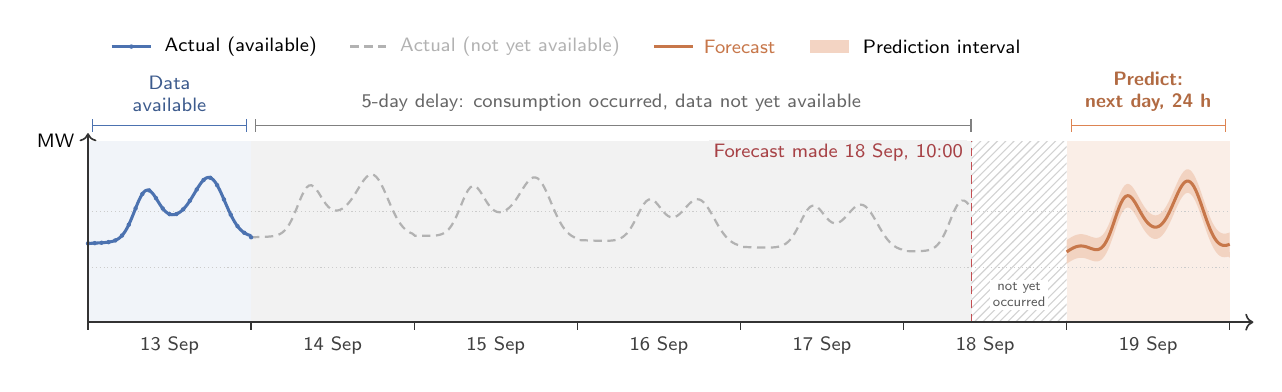
\begin{tikzpicture}[
  declare function={
    W = 14.5;                                     % chart width
    D = W/7;                                      % width of one day
    hr(\x) = 24*mod(\x,D)/D;                      % hour of day
    dw(\x) = floor(\x/D);                         % day index (0 = 13 Sep)
    we(\x) = ifthenelse(dw(\x)==3,1,ifthenelse(dw(\x)==4,1,0)); % 16--17 Sep = weekend
    mp(\x) = 8.5 + 2*we(\x);                      % morning peak later on weekends
    f(\x)  = 1.0 + 0.10*sin(360*\x/W)
             + (1-0.25*we(\x))*( 0.55*exp(-(hr(\x)-mp(\x))*(hr(\x)-mp(\x))/6)
                               + 0.70*exp(-(hr(\x)-18)*(hr(\x)-18)/10)
                               + 0.25*exp(-(hr(\x)-13)*(hr(\x)-13)/20) );
    g(\x)  = f(\x) + 0.07*sin(360*\x/(D/3)) - 0.03;  % illustrative forecast
    xi     = 5*D + 10*D/24;                       % forecast issued 18 Sep 10:00
  }]
  % Background regions
  \fill[cblue!8] (0,0) rectangle ({D},2.3);
  \fill[gray!10] ({D},0) rectangle (xi,2.3);
  \fill[pattern=north east lines, pattern color=gray!35] (xi,0) rectangle ({6*D},2.3);
  \fill[corange!14] ({6*D},0) rectangle ({7*D},2.3);
  \node[font=\tiny\sffamily, text=gray!70!black, align=center, fill=white, inner sep=1pt]
    at ({(xi+6*D)/2},0.35) {not yet\\occurred};
  % Region brackets and labels
  \begin{scope}[font=\scriptsize\sffamily]
    \draw[cblue, thin, |-|] (0.05,2.5) -- ({D-0.05},2.5);
    \node[anchor=south, text=cblue!80!black, align=center] at ({0.5*D},2.55) {Data\\available};
    \draw[gray, thin, |-|] ({D+0.05},2.5) -- (xi,2.5);
    \node[anchor=south, text=gray!80!black] at ({(D+xi)/2},2.55)
      {5-day delay: consumption occurred, data not yet available};
    \draw[corange, thin, |-|] ({6*D+0.05},2.5) -- ({7*D-0.05},2.5);
    \node[anchor=south, text=corange!80!black, font=\scriptsize\sffamily\bfseries, align=center]
      at ({6.5*D},2.55) {Predict:\\next day, 24 h};
  \end{scope}
  % Forecast issue time
  \draw[cred, densely dashed, line width=0.7pt] (xi,0) -- (xi,2.3);
  \node[anchor=south east, font=\scriptsize\sffamily, text=cred!85!black, fill=gray!10, inner sep=1.5pt]
    at ({xi-0.05},1.98) {Forecast made 18 Sep, 10:00};
  % Light horizontal grid
  \foreach \y in {0.7,1.4}
    \draw[gray!40, densely dotted] (0,\y) -- (W,\y);
  % Consumption that has occurred but is not yet available
  \draw[gray!60, line width=0.8pt, densely dashed]
    plot[domain={D}:xi, samples=300] (\x,{f(\x)});
  % Consumption available, with hourly markers
  \draw[cblue, line width=1.1pt] plot[domain=0:{D}, samples=100] (\x,{f(\x)});
  \foreach \k in {0,...,24}
    \fill[cblue] ({\k*D/24},{f(\k*D/24)}) circle (0.8pt);
  % Prediction interval and forecast for the target day
  \fill[corange, opacity=0.25]
    plot[domain={6*D}:{7*D}, samples=100] (\x,{g(\x)+0.15})
    -- plot[domain={7*D}:{6*D}, samples=100] (\x,{g(\x)-0.15}) -- cycle;
  \draw[corange!90!black, line width=1.1pt]
    plot[domain={6*D}:{7*D}, samples=100] (\x,{g(\x)});
  % Axes
  \draw[black!80, line width=0.6pt, ->] (0,0) -- ({W+0.3},0);
  \draw[black!80, line width=0.6pt, ->] (0,0) -- (0,2.4);
  \node[anchor=east, font=\scriptsize\sffamily] at (-0.05,2.3) {MW};
  \foreach \i in {0,...,7}
    \draw[black!80, line width=0.5pt] ({\i*D},0) -- ({\i*D},-0.1);
  \foreach \d [count=\i from 0] in {13 Sep,14 Sep,15 Sep,16 Sep,17 Sep,18 Sep,19 Sep}
    \node[font=\scriptsize\sffamily, text=black!75] at ({(\i+0.5)*D},-0.3) {\d};
  % Legend
  \begin{scope}[font=\scriptsize\sffamily]
    \draw[cblue, line width=1.1pt] (0.3,3.5) -- (0.8,3.5);
    \fill[cblue] (0.55,3.5) circle (0.8pt);
    \node[anchor=west] (l1) at (0.85,3.5) {Actual (available)};
    \draw[gray!60, line width=0.8pt, densely dashed] ($(l1.east)+(0.3,0)$) -- ++(0.5,0)
      node[anchor=west] (l2) {Actual (not yet available)};
    \draw[corange!90!black, line width=1.1pt] ($(l2.east)+(0.3,0)$) -- ++(0.5,0)
      node[anchor=west] (l3) {Forecast};
    \fill[corange, opacity=0.35] ($(l3.east)+(0.3,-0.08)$) rectangle ++(0.5,0.16);
    \node[anchor=west] at ($(l3.east)+(0.85,0)$) {Prediction interval};
  \end{scope}
\end{tikzpicture}
\caption{Information available when the forecast is made, illustrated with the example from the task description (synthetic curves). On 18 September at 10:00, measured consumption is only available up to 13 September because of the approximately 5-day data delay, and the remainder of 18 September has not yet occurred. The forecast must cover all 24 hours of 19 September, using historical consumption up to 13 September, the weather forecast for 19 September and calendar information.}
\label{fig:forecast-timeline}
\end{figure}

\subsection{Stakeholders}

The main stakeholders are:

\begin{description}[leftmargin=0pt, itemsep=3pt, parsep=0pt, topsep=4pt]
    \item[Aneo] Provides next-day hourly consumption forecasts for the retailer's six price areas.
    \item[Electricity retailer] Buys electricity in the day-ahead market and sells it to its customers with a mark-up.
    \item[End customers] Buy electricity as needed from their chosen electricity retailer.
    \item[Metering data hub (Elhub, Datahub)] Delivers metered consumption with a delay of about five days.
    \item[TSOs and eSett (Statnett, Fingrid)] Keep the system in balance and settle the retailer's imbalances.
\end{description}

\subsection{Value Chain and Objectives}
\label{sec:value-chain}

The forecasting service connects several actors, as shown in \cref{fig:actors}. Weather forecast providers supply Aneo with critical information such as temperature, humidity and wind, while metered consumption reaches Aneo through the metering data hubs with a delay of about five days. Based on this, Aneo delivers next-day hourly forecasts to the retailer, which uses them to nominate its expected demand in the day-ahead market. Any deviation between nominated and actual consumption is settled as an imbalance by the TSOs and eSett, and the cost is borne by the retailer.

\begin{figure}[H]
\centering
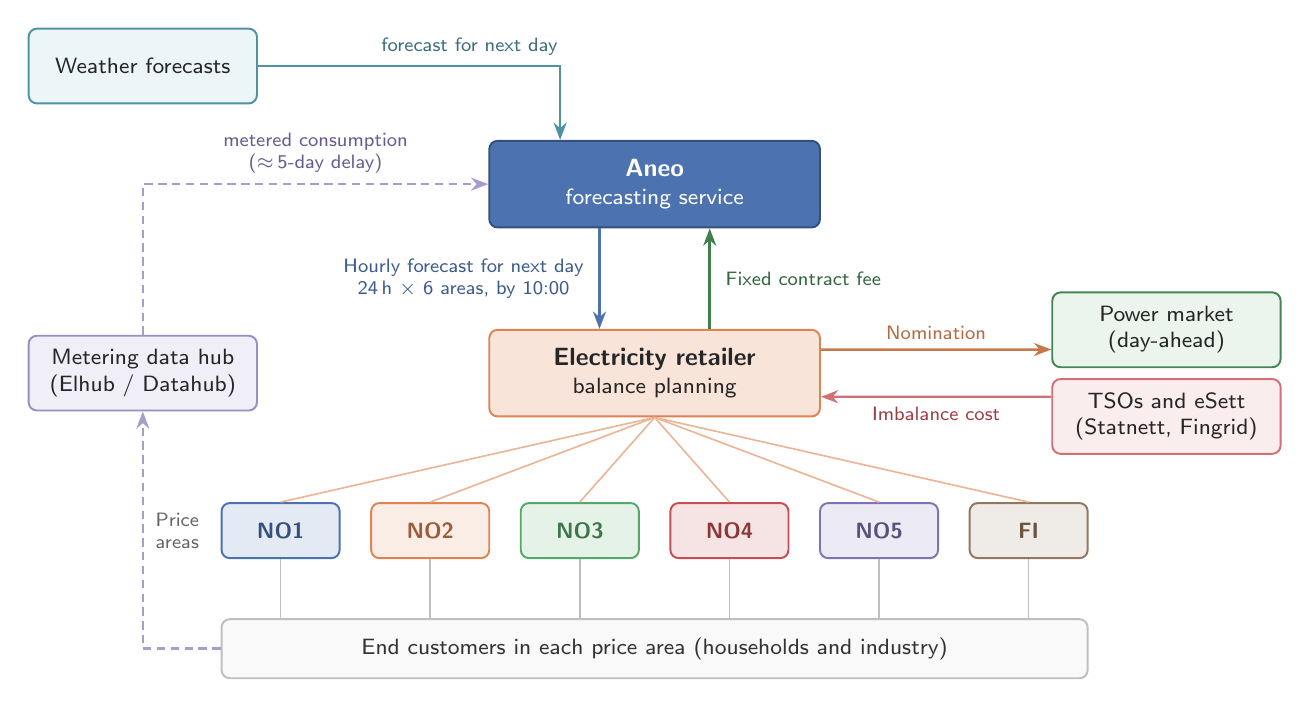
\begin{tikzpicture}[
  font=\small\sffamily,
  >={Stealth[length=2.2mm]},
  box/.style={rounded corners=3pt, align=center, inner sep=4pt, line width=0.7pt},
  aneo/.style={box, draw=cblue!70!black, fill=cblue, text=white, minimum width=4.2cm, minimum height=1.1cm, font=\small\sffamily\bfseries},
  retail/.style={box, draw=corange, fill=corange!22, text=black!85, minimum width=4.2cm, minimum height=1.1cm, font=\small\sffamily\bfseries},
  ext/.style={box, minimum width=2.9cm, minimum height=0.95cm, font=\footnotesize\sffamily, text=black!85},
  area/.style={box, minimum width=1.5cm, minimum height=0.7cm, font=\footnotesize\sffamily\bfseries},
  lbl/.style={font=\scriptsize\sffamily, align=center},
  flow/.style={->, line width=0.9pt},
  money/.style={->, cgreen!75!black, line width=0.9pt},
  data/.style={->, cpurple!70, line width=0.9pt, densely dashed},
]
  % Main actors
  \node[aneo] (aneo) at (0,5) {Aneo\\[-1pt]{\footnotesize\mdseries forecasting service}};
  \node[retail] (ret) at (0,2.6) {Electricity retailer\\[-1pt]{\footnotesize\mdseries balance planning}};
  \node[ext, draw=ccyan!80!black, fill=ccyan!12] (wx)  at (-6.5,6.5) {Weather forecasts};
  \node[ext, draw=cpurple!80, fill=cpurple!12] (hub) at (-6.5,2.6) {Metering data hub\\(Elhub / Datahub)};
  \node[ext, draw=cgreen!80!black, fill=cgreen!12] (mkt) at (6.5,3.15) {Power market\\(day-ahead)};
  \node[ext, draw=cred!80, fill=cred!10] (tso) at (6.5,2.05) {TSOs and eSett\\(Statnett, Fingrid)};

  % Price areas and customers
  \foreach \a/\c [count=\i from 0] in {NO1/cblue,NO2/corange,NO3/cgreen,NO4/cred,NO5/cpurple,FI/cbrown}
    \node[area, draw=\c, fill=\c!15, text=\c!70!black] (a\i) at ({-4.75+\i*1.9},0.6) {\a};
  \node[box, draw=gray!50, fill=gray!5, text=black!80, minimum width=11cm, minimum height=0.75cm,
        font=\footnotesize\sffamily] (cust) at (0,-0.9)
        {End customers in each price area (households and industry)};
  \foreach \i in {0,...,5} {
    \draw[corange!60, line width=0.6pt] (ret.south) -- (a\i.north);
    \draw[gray!50, line width=0.6pt] (a\i.south) -- (a\i.south |- cust.north);
  }
  \node[lbl, anchor=east, text=black!60] at ([xshift=-0.15cm]a0.west) {Price\\areas};

  % Flows between Aneo and retailer
  \draw[flow, cblue] ([xshift=-0.7cm]aneo.south) -- node[lbl, left, xshift=-2pt, text=cblue!80!black]
    {Hourly forecast for next day\\24\,h $\times$ 6 areas, by 10:00} ([xshift=-0.7cm]ret.north);
  \draw[money] ([xshift=0.7cm]ret.north) -- node[lbl, right, xshift=2pt, text=cgreen!60!black]
    {Fixed contract fee} ([xshift=0.7cm]aneo.south);

  % Inputs to Aneo
  \draw[flow, ccyan!80!black] (wx.east) -| node[lbl, above, pos=0.35, text=ccyan!60!black] {forecast for next day} ([xshift=-1.2cm]aneo.north);
  \draw[data] (cust.west) -| (hub.south);
  \draw[data] (hub.north) |- node[lbl, above, pos=0.75, text=cpurple!80!black]
    {metered consumption\\($\approx$\,5-day delay)} (aneo.west);

  % Retailer and market
  \draw[flow, corange!90!black] ([yshift=0.3cm]ret.east) -- node[lbl, above, text=corange!80!black] {Nomination}
    ([yshift=-0.25cm]mkt.west);
  \draw[flow, cred!80] ([yshift=0.25cm]tso.west) -- node[lbl, below, text=cred!80!black] {Imbalance cost}
    ([yshift=-0.3cm]ret.east);

\end{tikzpicture}
\caption{Actors and flows in the case. Aneo delivers next-day consumption forecasts to the retailer, which uses them to nominate demand and bears the imbalance cost.}
\label{fig:actors}
\end{figure}

The quality of the input data is crucial, since a predictive model is only as good as the data it is based on. Errors in the weather forecasts propagate through the whole chain: Aneo's predictions become less accurate, which means that the electricity retailer must settle the resulting deficit or surplus at less favourable imbalance prices, reducing its profit.

Errors can also come from the consumption data, for example missing or delayed meter values, or from changes in the retailer's customer portfolio that the model does not capture. Aneo can also be affected by a poor predictive model: even if the weather forecasts are accurate, the forecasts delivered to the retailer will be wrong if the model uses this information incorrectly. An example could be failing to rank the importance of each source, leading to a wrong combination or formula. Customers are also affected, although only indirectly: if imbalance costs remain high over time, the retailer may pass some of them on through higher prices, which in turn can lead customers to switch to another retailer.

Since the retailer pays Aneo a fixed fee, Aneo does not earn or lose money directly from each imbalance. Instead, the value of the service lies in how it affects the retailer, as illustrated in \cref{fig:value-chain}. More accurate forecasts reduce the retailer's imbalance and financial exposure, which increases the perceived value of the service and the retailer's willingness to pay for it. For Aneo, this ultimately translates into customer satisfaction and a higher likelihood of contract renewal.

\begin{figure}[H]
\centering
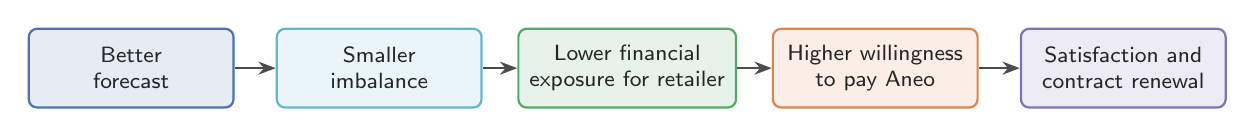
\begin{tikzpicture}[
  >={Stealth[length=2.2mm]},
  chain/.style={rounded corners=3pt, align=center, text=black!85,
                inner sep=4pt, line width=0.8pt, minimum width=2.6cm, minimum height=1cm,
                font=\footnotesize\sffamily},
  flow/.style={->, black!70, line width=0.8pt},
]
  \foreach \t/\c [count=\i from 0] in {Better\\forecast/cblue, Smaller\\imbalance/ccyan, Lower financial\\exposure for retailer/cgreen,
                                       Higher willingness\\to pay Aneo/corange, Satisfaction and\\contract renewal/cpurple}
    \node[chain, draw=\c, fill=\c!14] (c\i) at ({\i*3.15},0) {\t};
  \foreach \i [evaluate=\i as \j using int(\i+1)] in {0,...,3}
    \draw[flow] (c\i.east) -- (c\j.west);
\end{tikzpicture}
\caption{Value chain for Aneo. Because Aneo is paid a fixed fee, forecast quality creates value indirectly, through the retailer's willingness to pay for the service and the likelihood of contract renewal.}
\label{fig:value-chain}
\end{figure}

Based on this, the project has three main objectives:

\begin{description}[leftmargin=0pt, itemsep=2pt]
    \item[Technical] Produce accurate and unbiased hourly forecasts that outperform a simple baseline in all six price areas.
    \item[Business] Reduce the retailer's total imbalance and the frequency of large forecast errors.
    \item[Operational] Deliver the forecasts reliably before 10:00 every day, using only information available at that time.
\end{description}

The measurable criteria used to evaluate these objectives are defined in \cref{sec:success}.

\subsection{Success Criteria}
\label{sec:success}

The objectives in \cref{sec:value-chain} are evaluated on a held-out test period that the models have not seen during training or tuning (see \cref{sec:validation}).

\begin{description}[leftmargin=0pt, itemsep=2pt]
    \item[Technical] Lower mean absolute error (MAE) than the same-hour-last-week baseline in all six price areas, and a bias close to zero. The choice of MAE as the main measure is justified in \cref{sec:metrics}.
    \item[Business] Lower total imbalance (MWh) and fewer hours with large errors than the baseline, consistently across price areas and seasons. Specific target levels would in practice be agreed with Aneo and the retailer, for example in a service-level agreement.
    \item[Operational] The forecast is produced before 10:00 every day, using only data available at that time.
\end{description}

\subsection{Constraints and Assumptions}

The main constraints are that the forecast is issued at around 10:00 for the next day, that consumption data are only available up to five days earlier, and that only temperature forecasts and calendar information are available as additional inputs (see \cref{sec:decision}). We further assume that:

\begin{itemize}[itemsep=0pt, topsep=4pt]
    \item the retailer pays Aneo a fixed fee, and over- and underforecasting are equally costly;
    \item imbalance costs scale approximately linearly with the forecast error, so the full settlement mechanism is not modelled;
    \item the temperature values are forecasts available at the time the consumption forecast is made;
    \item Aneo's current forecasting method is unknown, so a simple baseline is used as the reference.
    \item the retailer is small relative to each price area, so its forecast errors do not affect the imbalance price;
    \item the external weather data, which are observed values, are used as an approximation of weather forecasts;
    \item the retailer nominates directly based on the forecast, without later adjustments in the intraday market.
\end{itemize}
\newpage

% =====================================================================
\section{Data Understanding and Background}
\label{sec:data}
\subsection{Domain Background}
The electricity market divides Norway into 5 different price-regions, while Finland is kept as one big price region. Supply and Demand within each region combined with possible trade between price regions, depending on transmission capacity dictates a market price for each delivery interval (currently one hour, but will move towards 15-minutes intervals), the day ahead. The consumption values represent only the retailer's customers in each price area, not the total consumption in that area. Therefore consumption of the customers can be dependent on a different mix of variables than that of the price region as a whole.


One of the biggest consumers of electricity is heating. Norway and Finland are both located in cold climates where heating is a necessity, especially in the winter months. Especially households have a higher consumption of electricity in the winter due to heating, thus temperature is a key input-variable for forecasting demand. Consumption also follows daily patterns. When the population wakes up, lights are turned on, showers use warm water that needs to be replenished etc and drives up demand. During the working day, industry is driving the demand, while households are driving the demand again in the evening cooking, doing laundry etc. During the night, activity falls and so does the power consumption. Thus, time information, such as the hour of the day and day of the week, are important input variables for forecasting electricity demand.

The retailer submits bids in the day-ahead market on Nord Pool for the price regions in which it operates. Accepted bids are binding, although the retailer can adjust its purchases through intraday trading before delivery. Since electricity production and consumption must remain balanced, the TSOs use balancing markets to address differences between planned and actual production and consumption. The retailer bears financial responsibility for deviations between its contracted purchases and its customers’ actual consumption, either directly as a balance responsible party or through an agreement with one. These deviations are settled at the imbalance price, which can differ from the day-ahead price. Forecast errors can therefore cause financial losses for the retailer.

Public holidays may also affect electricity consumption by changing household routines and business activity. However, our dataset covers only one year, providing limited examples from which to learn holiday effects. These effects may therefore be difficult to distinguish from other influences, such as temperature and day of the week.

\subsection{Dataset Description}
The dataset \texttt{consumption\_temp.csv} contains 49,494 hourly
observations across five locations in Norway and one in Finland. Each row
contains four variables: \texttt{time}, the timestamp in UTC;
\texttt{location}, the location identifier; \texttt{consumption},
the average electricity demand during the hour in MW; and
\texttt{temperature}, the forecast temperature in $^\circ$C.
An average demand of 1 MW over one hour corresponds to an energy
consumption of 1 MWh.

The Norwegian locations cover the period from 7 April 2022 at
21:00 to 2 April 2023 at 21:00, with 8,641 observations per
location. Finland, labelled \texttt{helsingfors} in the dataset,
starts on 14 July 2022 at 21:00 and ends at the same time as the
Norwegian series, giving 6,289 observations.

Table~\ref{tab:dataset_locations} shows the location identifiers
and their corresponding electricity price areas. The consumption series represent the retailer's customers associated with each location, rather than total consumption in the price area. As a result, the consumption level depends on how many customers the retailer serves in each area rather than on the size of the representative city, so levels cannot be compared directly across areas. The level may also change abruptly if the retailer gains or loses customers, which a model may mistake for a change in demand.

\begin{table}[htbp]
    \centering
        \caption{Locations, corresponding price areas and observation counts.}
    \label{tab:dataset_locations}
    \begin{tabular}{llr}
        \hline
        Location & Price area & Observations \\
        \hline
        Oslo       & NO1 & 8,641 \\
        Stavanger  & NO2 & 8,641 \\
        Trondheim  & NO3 & 8,641 \\
        Troms{\o}  & NO4 & 8,641 \\
        Bergen     & NO5 & 8,641 \\
        Helsingfors & FI & 6,289 \\
        \hline
        Total & & 49,494 \\
        \hline
    \end{tabular}

\end{table}
\subsection{Exploratory Data Analysis}
\label{sec:eda}

The exploratory analysis focuses on the patterns that motivate the choice of features and models in \cref{sec:methods}.

\paragraph{Consumption level and seasonality}\mbox{}\\
The consumption level differs considerably between locations, with Oslo having the highest and Tromsø the lowest across the whole year. Because of these differences in level, forecast errors are also compared relative to the consumption level (nMAE) in \cref{sec:methods}. All Norwegian locations show a strong seasonal pattern: in Oslo, the monthly mean rises from about 2.3\,MW in the summer of 2022 to about 13.4\,MW in December 2022 (\cref{fig:consumption-level}).

Not all of this increase is seasonal, however. At similar temperatures, Norwegian consumption in October 2022 is roughly 1.3 to 2 times the level in April 2022; in Oslo, for example, the mean is 2.8\,MW at 7.6\,$^\circ$C in April and 6.1\,MW at 8.1\,$^\circ$C in October. In Helsinki, consumption increases from about 2.6 to 6.3\,MW between July and September 2022. Since temperature alone cannot explain these level shifts, they most likely reflect changes in the retailer's customer portfolio. Lagged consumption features can capture such shifts, while temperature cannot.


\begin{figure}[htbp]
\centering
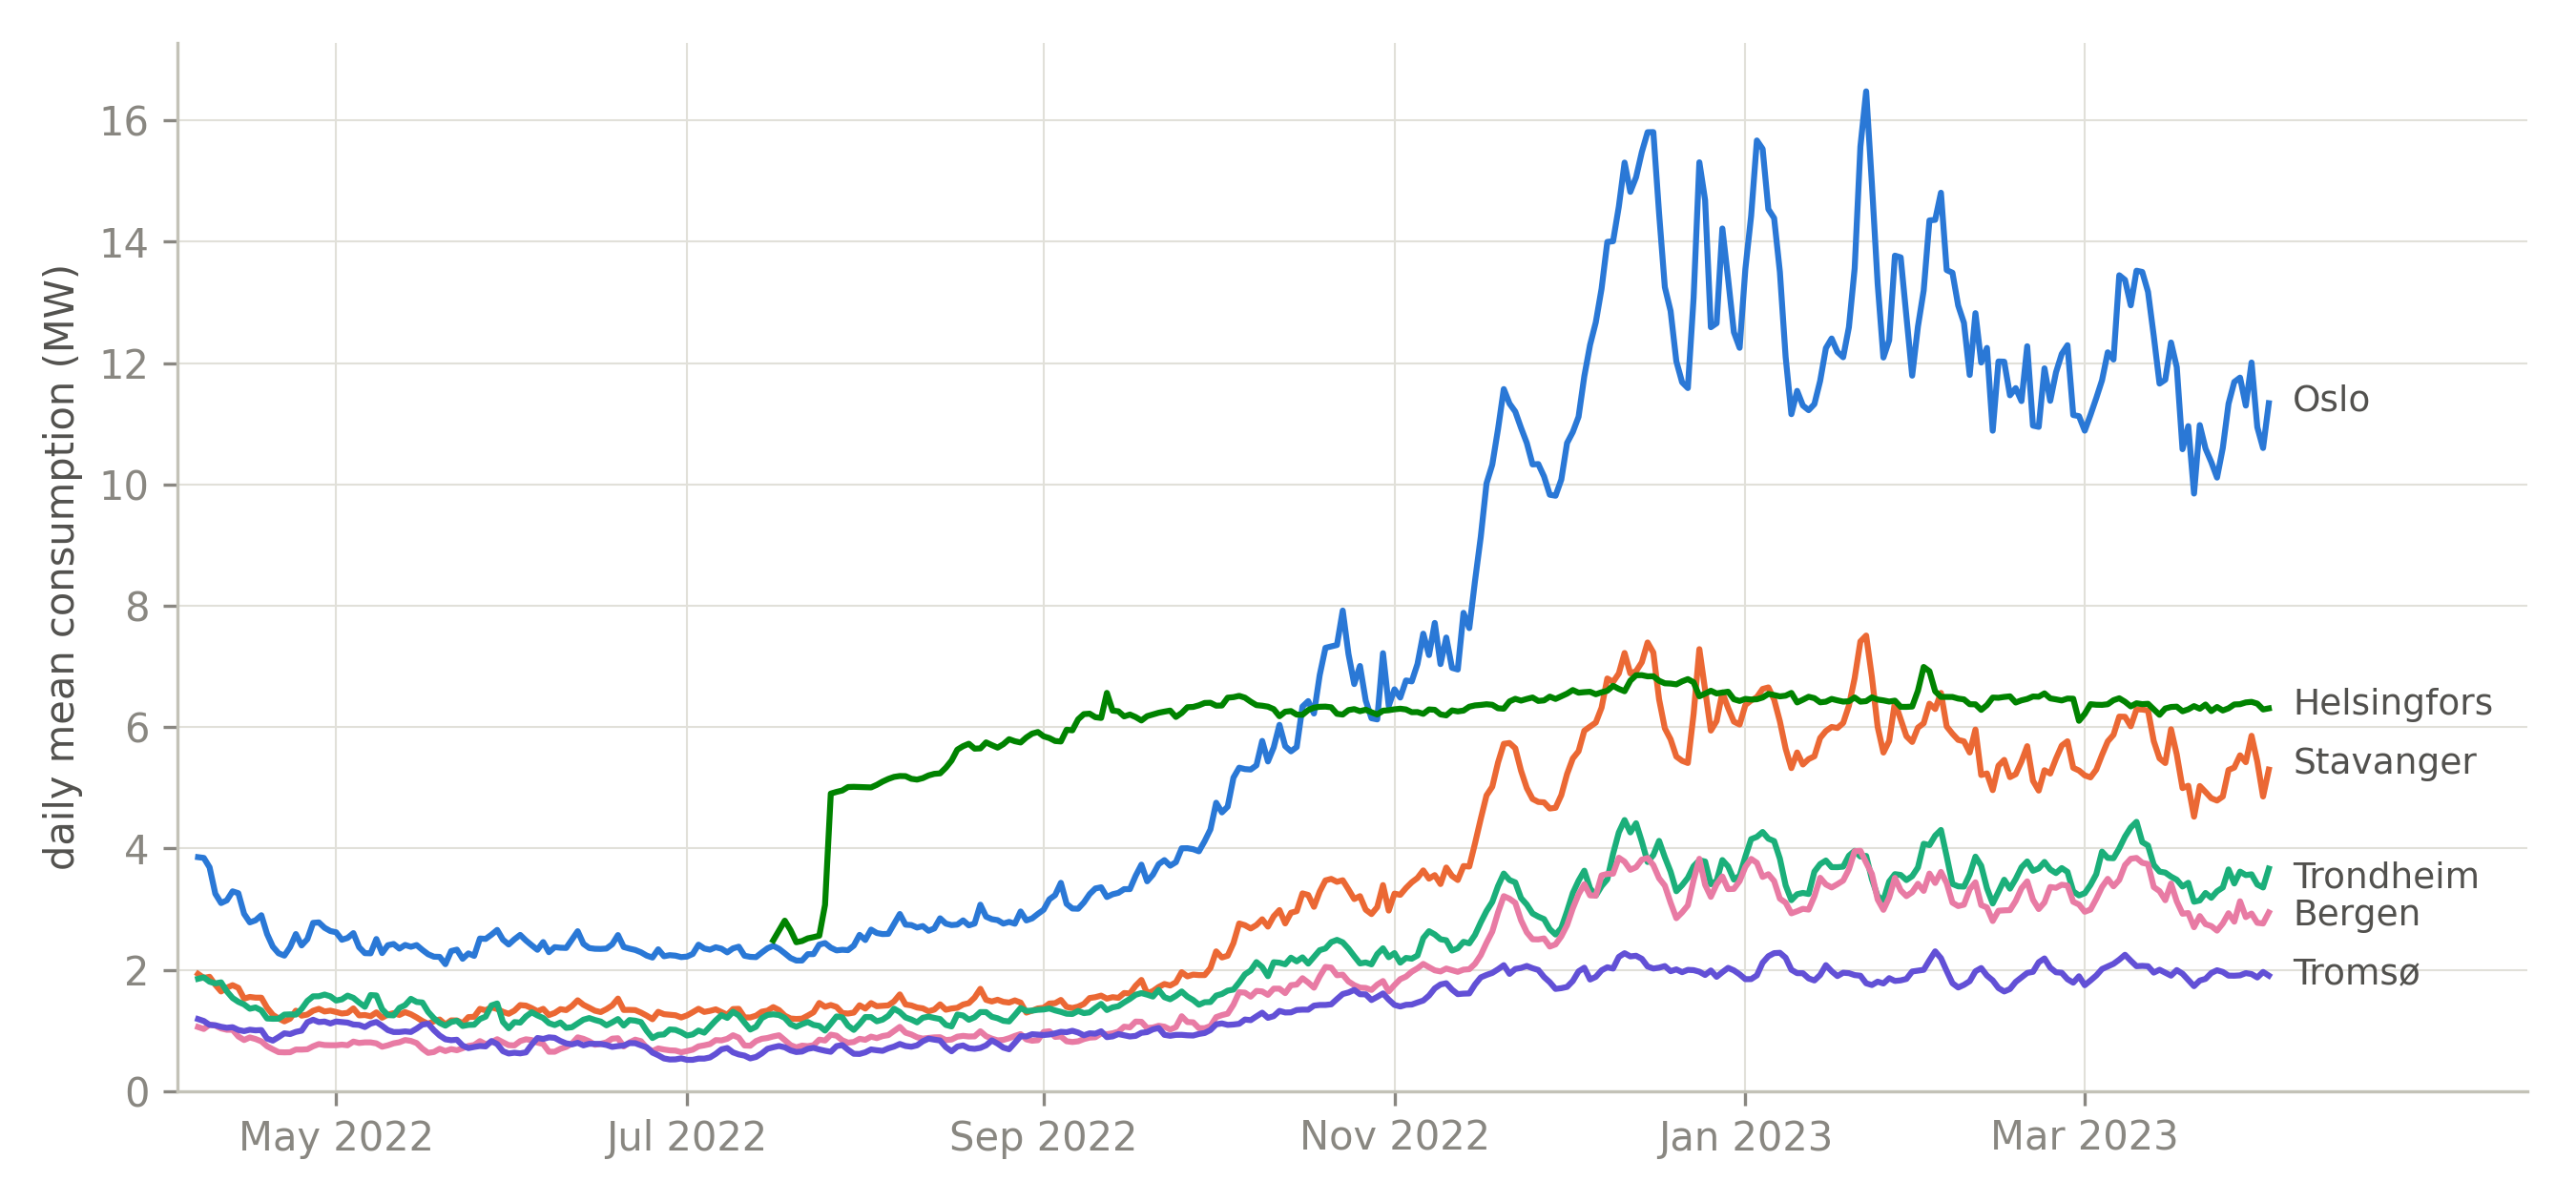
\includegraphics[width=0.9\linewidth]{figures/2 Data Understanding and Background/consumption_level.png}
\caption{Daily mean consumption per location. The levels differ considerably, and all Norwegian locations rise sharply from October. The Finnish series starts in July 2022 and jumps from about 2.6 to 5\,MW within a few days.}
\label{fig:consumption-level}
\end{figure}

\paragraph{Consumption and temperature}\mbox{}\\
Within each location, consumption and temperature are strongly negatively correlated, with correlation coefficients between $-0.78$ and $-0.86$ for the Norwegian locations and $-0.60$ for Helsinki. The relationship is non-linear: consumption is almost flat above about 10--12\,$^\circ$C and increases steeply below, which is consistent with a heating threshold. This makes temperature the most important explanatory variable and motivates models that can capture non-linear effects. \cref{fig:temp-scatter} shows the relationship per location.

\begin{figure}[htbp]
\centering
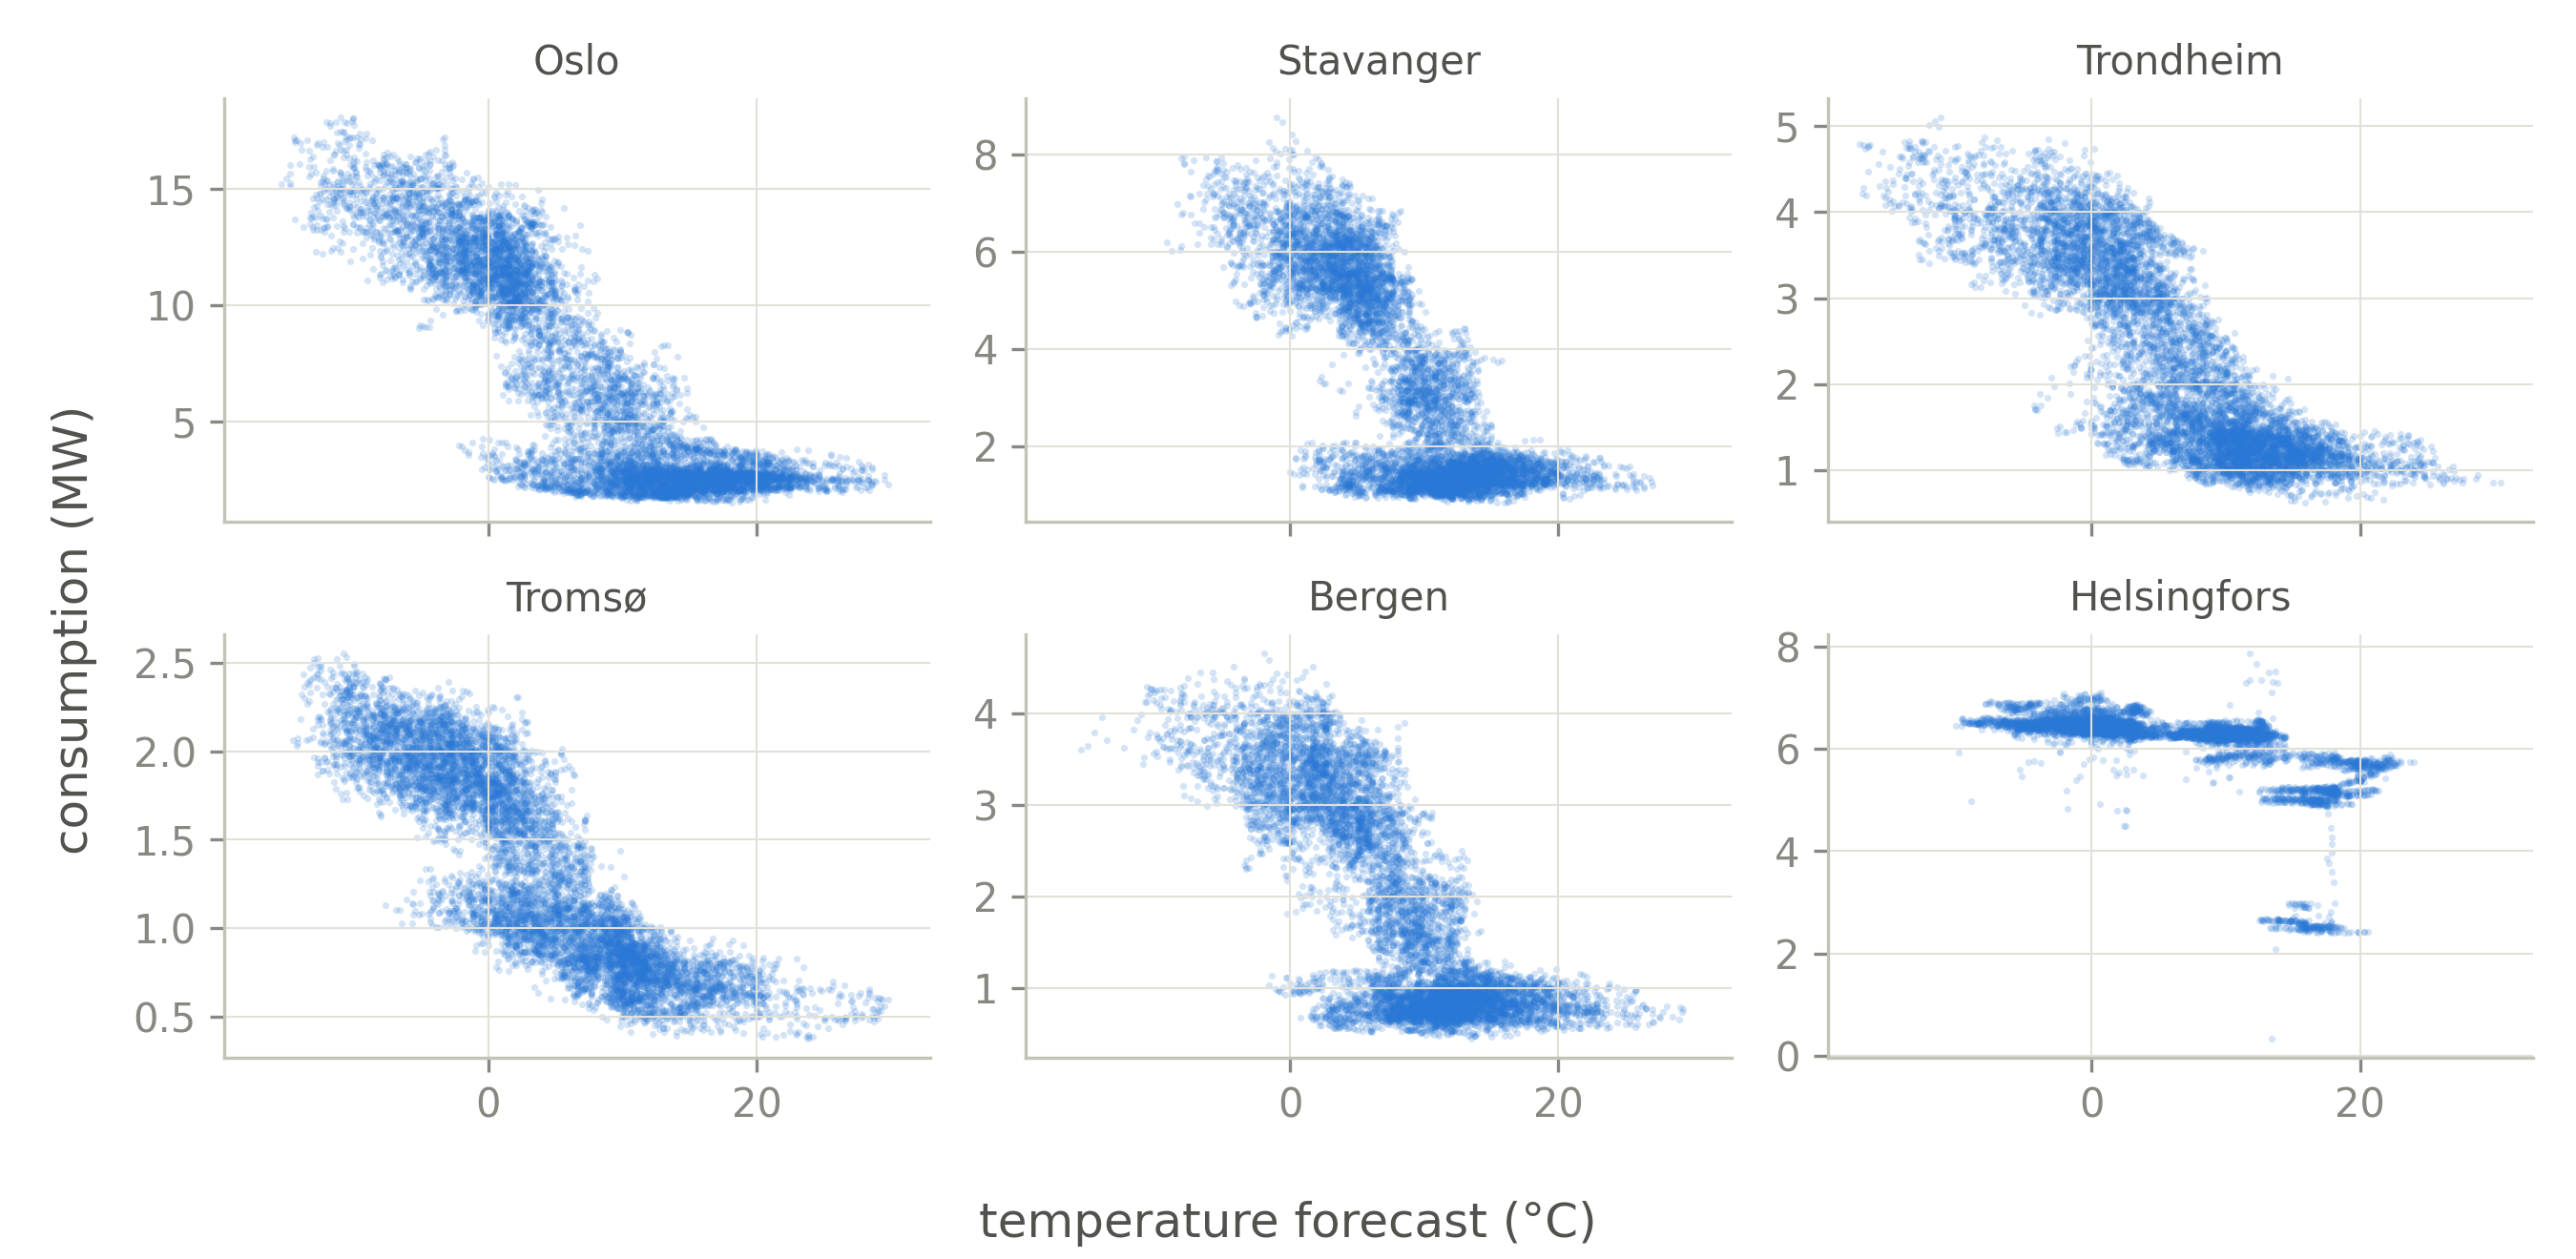
\includegraphics[width=0.8\linewidth]{figures/2 Data Understanding and Background/temperature_scatter.png}
\caption{Hourly consumption against temperature forecast per location. Consumption is nearly flat at high temperatures and rises steeply below roughly 10\,$^\circ$C. The separate low-consumption cluster at the same temperatures is the period before the level shift in autumn 2022 (see \cref{fig:consumption-level}). Note the different y-axis scales.}
\label{fig:temp-scatter}
\end{figure}

\paragraph{Daily and weekly patterns}\mbox{}\\
The daily profile is clearly shaped by the time of day and by whether it is a weekday or weekend. On weekdays, consumption has a morning peak around 07:00, a dip during the working day and a larger evening peak at around 20:00. On weekends the morning peak is replaced by a later and broader rise from about 09:00, and the evening peak is slightly higher. Consumption is lowest at night in all Norwegian locations. Helsinki is almost flat over the day with no clear weekend effect, which suggests that its portfolio differs from the Norwegian ones. These patterns motivate hour-of-day, weekday and weekend features, and show that the hour of day and the day type interact. \cref{fig:daily-profiles} shows the average profiles.

\begin{figure}[htbp]
\centering
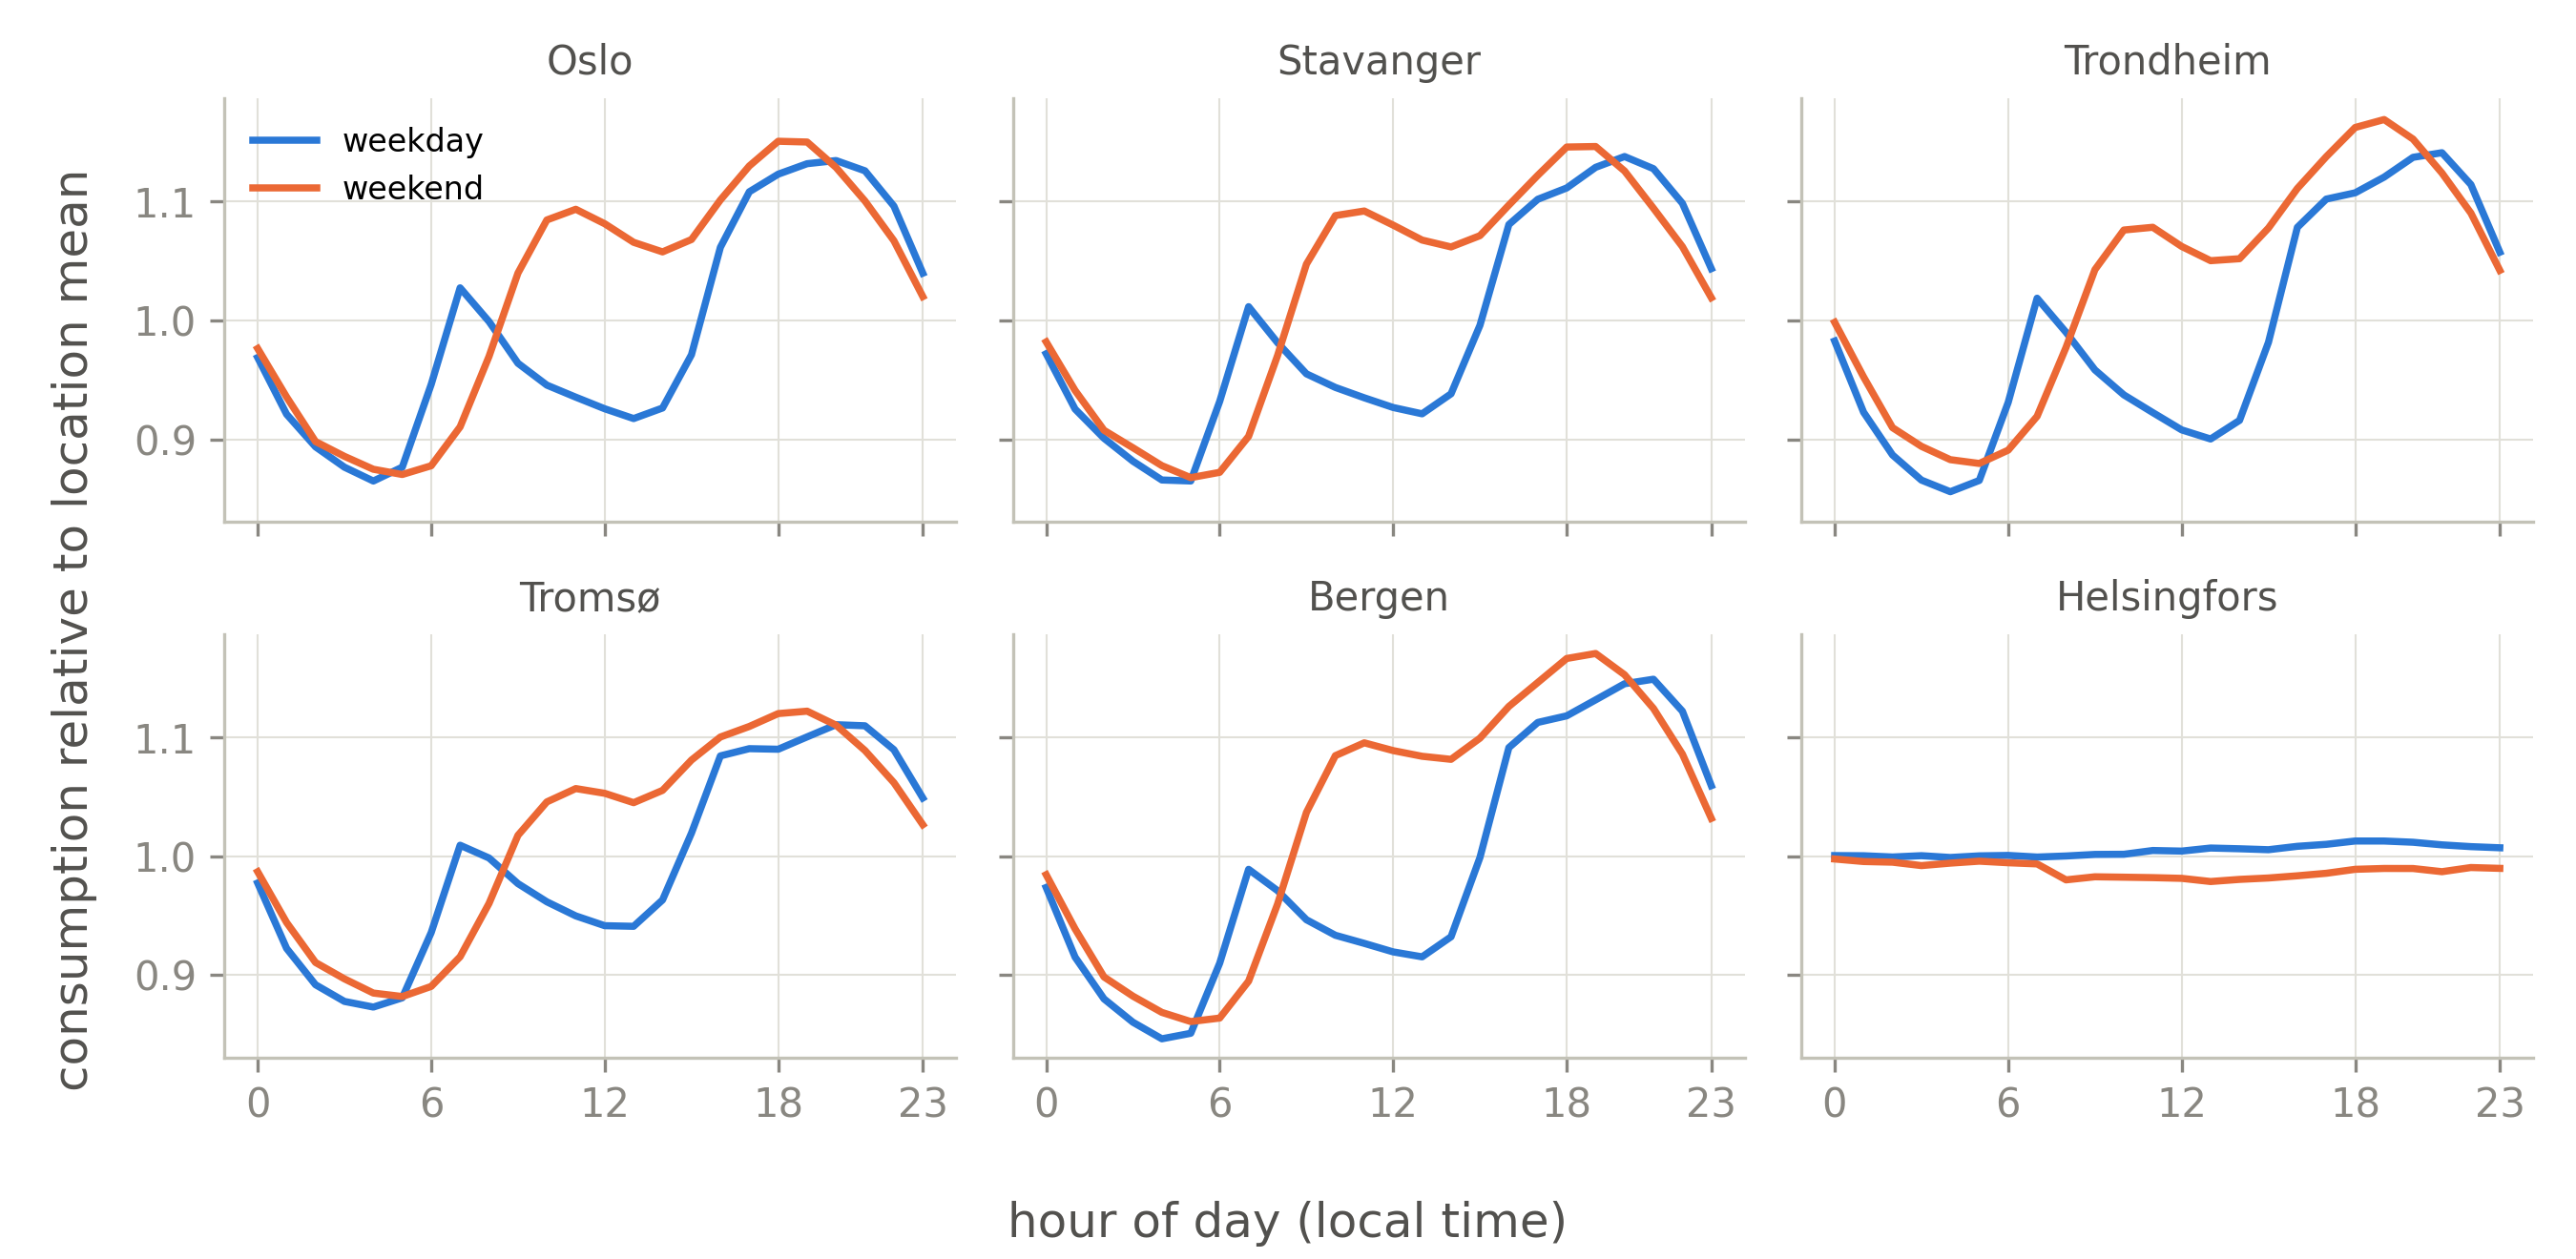
\includegraphics[width=0.8\linewidth]{figures/2 Data Understanding and Background/daily_profiles.png}
\caption{Average daily consumption profile per location, shown relative to each location's mean and in local time, for weekdays and weekends. Norwegian locations have a morning peak on weekdays that is delayed on weekends and an evening peak that is earlier on weekends. Helsingfors is nearly flat.}
\label{fig:daily-profiles}
\end{figure}

\FloatBarrier
\subsection{Data Quality Issues}

\todo{Points to cover (the sentence on missing values and duplicates in 2.2 could be moved here):}
\begin{itemize}[itemsep=0pt, topsep=2pt]\color{red}
    \item The Finnish series starts about three months later, so less training data is available for Finland.
    \item Timestamps are in UTC, so local time (including daylight saving time) must be derived for calendar features.
    \item Any outliers or level shifts found in the exploratory analysis, and how they are handled.
    \item The temperature values are forecasts and contain their own errors.
\end{itemize}

An analysis of the data shows that the data are of really good Quality. There are no missing data, duplicates or "gaps", there are however some limitations worth noting. As previously mentioned the data for Finland starts at a later point and have 27.2\% fewer data points. This gives the finish power region less training data for our model. The first 32 hours of the finish data also have consumption set to 0. While it might seem like an error, it makes sense as maybe the retailer started serving finish customers at this point. Other than that the dataset is complete.

The data is using UTC-time, while this standardizes nicely, it is worth noting that Finland and Norway uses different time-zones. Norway uses UTC+1 while Finland uses UTC+2, both countries also uses daylight saving time (UTC+2 and UTC+3 corresponding). This means that 7 am in the dataset corresponds to a different local time for Norway and Finland. For training it's necessary to derive local time through calendars. 

Since timestamps are stored in UTC, daylight-saving transitions introduce no gaps or duplicate timestamps in the dataset. However, converting to local time produces days with 23 or 25 hourly observations, which matters when interpreting daily patterns and constructing calendar features.

The temperature data in consumption.csv is the forecast that 

\subsection{Possible External Data}
\todo{Points to cover (consider renaming to ``External Data'', since external data have actually been used, and describe what was used rather than what is possible):}
\begin{itemize}[itemsep=0pt, topsep=2pt]\color{red}
    \item Wind and precipitation per location: the source, and whether these are forecasts or observed weather. If observed, this must be stated as a limitation.
    \item Holiday calendars for Norway and Finland.
    \item Possibly prices, if they are retrieved for the business evaluation.
\end{itemize}

\subsection{Assumptions and Limitations}
\todo{Points to cover (keep this to limitations of the data, so it does not overlap with Section 1.6):}
\begin{itemize}[itemsep=0pt, topsep=2pt]\color{red}
    \item Only about one year of data, so each season and each public holiday occurs only once.
    \item One city represents the weather for the whole price area.
    \item No customer-level data, so portfolio changes cannot be observed directly.
    \item If the weather data are observed values: the results may be somewhat optimistic.
\end{itemize}

\newpage

% =====================================================================
% Ansvarlig: Thomas & Truls
\section{Methods, Analysis and Technical Evaluation}
\label{sec:methods}
\subsection{Reproducing the Forecasting Situation}
As stated in the task description, consumption measurements are available with a delay of approximately five days. When the forecast for 19 September is made at 10:00 on 18 September, the most recent consumption data are therefore from 13 September (see \cref{fig:forecast-timeline}). Weather forecasts and calendar information, on the other hand, are available for the day being predicted.

\subsection{Data Processing}
Prior to training our models, we prepare the data by converting all dates into pd.datetime objects, and then to UTC for the datasets used. As a part of our data exploration we found there were no missing values in the dataset, and no need to handle NAs there. However, there is still a possibility of missing values at inference time, and we need a protocol to handle these events. Calendar features (hour, weekday, holiday) are deterministic and cannot be missing. The realistic failures are of two kinds, with different causes: (i) the consumption lags and the min/max of the last available day, which depend on the metering data hub and its five-day delay, and (ii) the weather features, which all come from one provider and therefore tend to be missing together.

\begin{figure}[H]
\centering
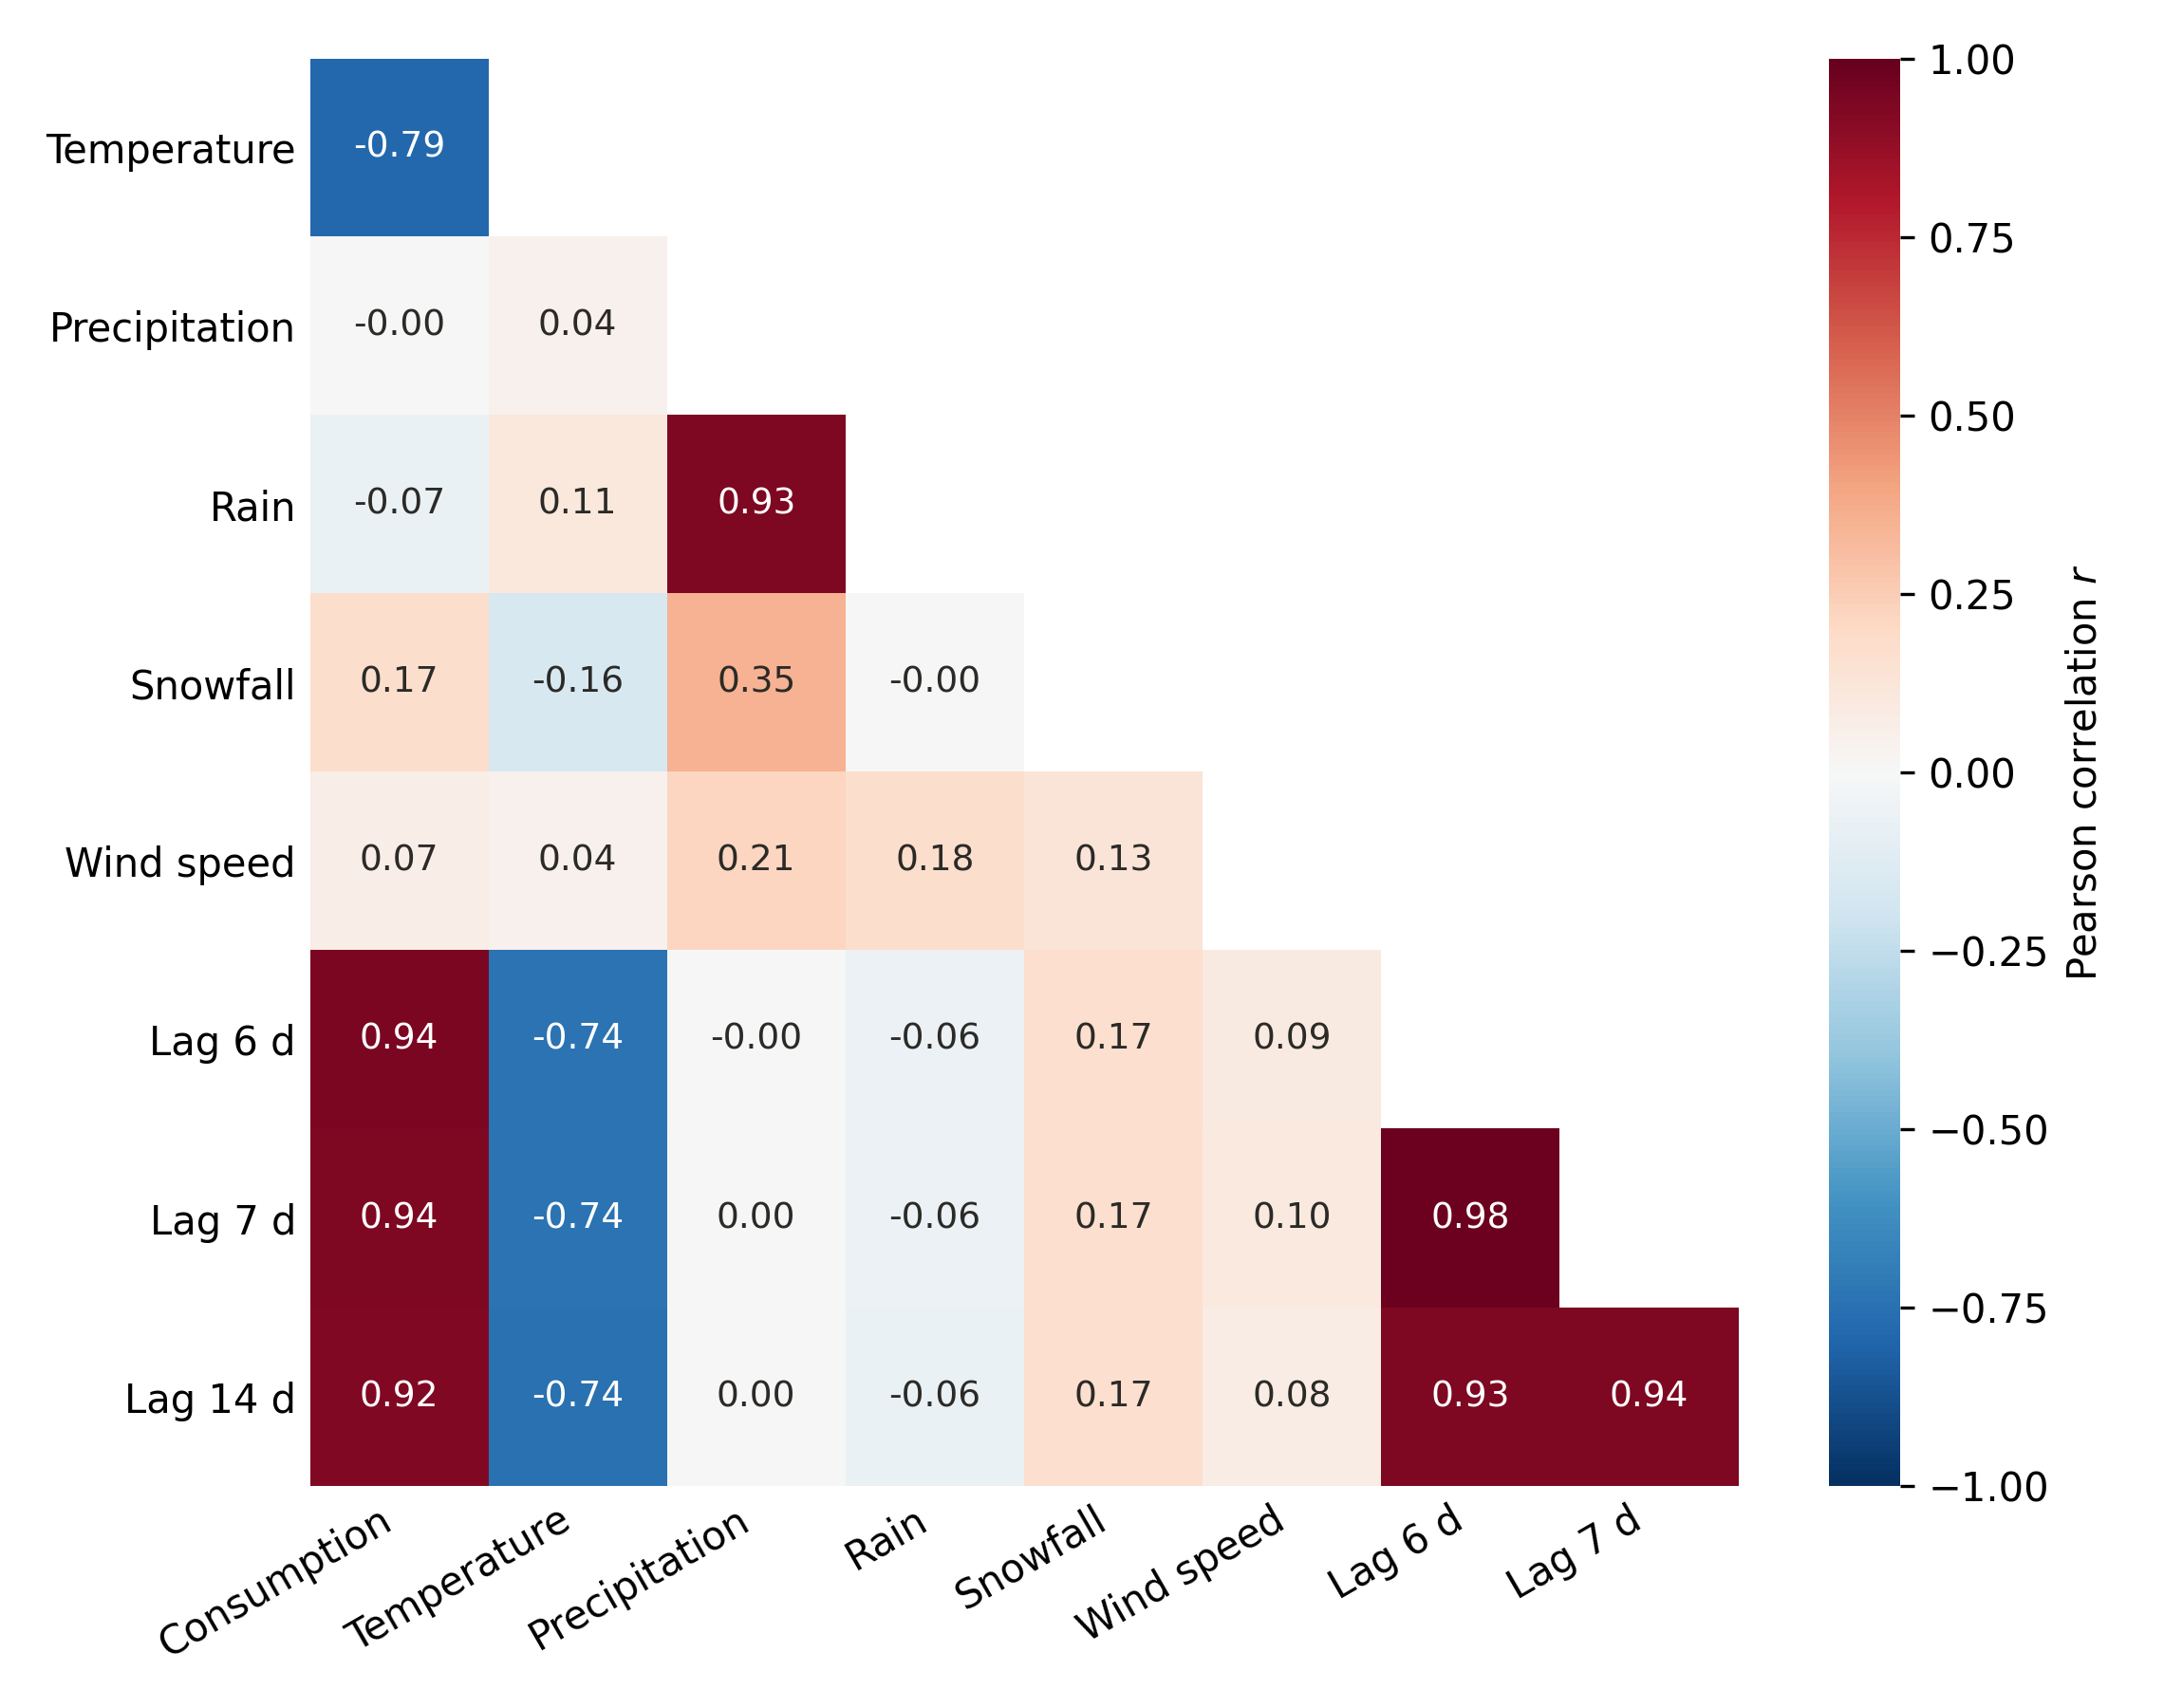
\includegraphics[width=0.65\linewidth]{figures/3 Methods, Analysis and Technical Evaluation/attribute_correlation_heatmap.png}
\caption{Pearson correlation between the attributes, computed within each location and then averaged over the locations. Computing it within locations avoids the level differences between the cities inflating or masking the correlations.}
\label{fig:attribute-correlation}
\end{figure}

\subsubsection*{How the correlations motivate the methods}
A value can only be imputed from other features that are correlated with it, so \cref{fig:attribute-correlation} tells us which methods are worth testing. The consumption lags are very strongly correlated with each other ($r = 0.93$--$0.98$) and with consumption ($r = 0.92$--$0.94$), so a missing lag can be predicted from the others; this motivates regression-based imputation (MICE, where each feature is regressed on all the others) against simple alternatives such as KNN and mean imputation. The weather variables are only weakly correlated with each other (temperature has $|r| \le 0.16$ to the rest), so a missing temperature cannot be recovered from them, and we use interpolation and persistence instead. If all consumption features are missing, the strongest remaining signal is temperature ($r = -0.79$), which motivates a model on weather and calendar only. Pearson correlation only captures linear relationships, and temperature and consumption are related non-linearly, so the correlations guide which methods to test, while the experiment decides which works.

\subsubsection*{Protocol and experimental set-up}
The resulting protocol, applied per row (\texttt{machine\_learning/imputation.py}): (1) weather gaps of up to three hours are interpolated, and longer gaps are filled with the value from the same hour the day before, then the training mean; (2) if at most four of the five consumption lag features are missing, they are imputed with MICE (scikit-learn's \texttt{IterativeImputer}); (3) if all are missing, the forecast comes from a second model trained on weather and calendar features only.

We tested it on the chronological split used for all models (training 7 April 2022--14 January 2023, 38,235 rows; test 20 January--3 April 2023, 10,495 rows; a six-day gap for the consumption delay). The imputation models are fitted on the training period only, and the forecasting model is XGBoost (500 trees, learning rate 0.05, depth 5, one of the grid-search combinations). Outages are simulated by removing whole days of data for 20\,\% of the (location, day) pairs in the test period, the same days for all methods, and the MAE is measured on the affected hours.

\subsubsection*{Results}
\cref{tab:missing-data} shows the MAE for the four outage scenarios; without any outage it is 0.38\,MW on the same hours. The full comparison with all methods we tried is in \cref{app:missing-data}.

\begin{table}[H]
\centering
\caption{MAE [MW] on the hours affected by a simulated outage (lowest in bold). All methods tried are in \cref{tab:missing-data-full}.}
\label{tab:missing-data}
\small
\setlength{\tabcolsep}{4pt}
\begin{tabularx}{\textwidth}{X *{4}{>{\centering\arraybackslash}p{2.3cm}}}
\toprule
 & Lag 7 d missing & Last available day missing & All consumption features missing & Whole weather forecast missing \\
\midrule
XGBoost, NaN handled natively & 0.70 & 2.77 & 3.92 & 0.62 \\
Mean imputation & 0.40 & 2.56 & 3.05 & 0.63 \\
KNN imputation ($k=5$) & 0.39 & 0.57 & 2.57 & 0.69 \\
MICE & \textbf{0.38} & \textbf{0.40} & 2.99 & \textbf{0.44} \\
Trained with outages & 0.43 & \textbf{0.40} & 1.67 & 0.57 \\
\textbf{Proposed:} MICE + weather model & \textbf{0.38} & \textbf{0.40} & \textbf{0.89} & \textbf{0.44} \\
Baseline (same hour last week) & 2.79 & 0.57 & 2.79 & 0.57 \\
\bottomrule
\end{tabularx}
\end{table}

\noindent The results follow the correlation structure. Methods that exploit the correlation between the lags are within 0.02\,MW of the error without outage when lags are missing, while native NaN handling and mean imputation are far worse when the last available day is missing (2.6--2.8\,MW). For weather, interpolation and persistence (0.44\,MW) beat KNN, mean and native NaN handling (0.62--0.69\,MW). When all consumption features are missing the error more than doubles to 0.89\,MW, but this is much better than the baseline or a fixed profile (2.79\,MW), because temperature explains much of the variation. Variants of MICE (ExtraTrees, multiple imputation) differ by at most 0.03\,MW, so we use the simplest. Training with simulated outages helps, but is not as good as imputing, and one model per pattern of missing features matches the proposed protocol but needs several models. The limit of four missing lags comes from removing $k$ of the five lags at random: MICE beats the weather and calendar model for $k \le 4$ (0.38--0.41 against 0.89\,MW) but not for $k=5$ (3.0\,MW, \cref{tab:threshold}). The test uses randomly placed single-day outages, so longer real outages may be harder to handle.

\subsection{Feature Engineering}
In order to increase the model performance, we tried to perform extensive feature engineering. Our effort was focusing using logical relations in the data to build the features, such as adding an attribute for season, whether it is weekday or weekend. When deciding on which features to keep we followed two criteria:
1. The engineered attribute must have a significant correlation to the consumption,
2. The engineered attribute must be practical to implement.
We decided against adding Season into the final model, as it is not practical. The reason is that we only have about 1 year of training data. Thus, the model would only see the season attribute for one year, meaninging we have just one summer, one winter, one spring and one autumn.

Some engineered attributes that were strongly correlated to the target (consumption) was the consumption on the same hour 6 days ago, 7 days ago and 14 days ago. In addition, we saw that temperature is highly correlated to the consumption, thus we decided to explore what other weather data is correlated to consumption. Weather data was extracted from OpenMetro.
\begin{figure}
        \centering
        \includegraphics[width=0.75\linewidth]{correlation_to_consumption.png}
        \caption{Correlation between attributes and consumption in five days}
    \label{fig:placeholder}
\end{figure}

Our findings were interesting. Weekday and Weekend had little correlative power and was thus removed from the model, this was against our hypothesis that there is a meaningfull difference in consumption patterns between weekdays and weekends. Likewise, we were surpised that wind direction has a larger impact than wind speed. This most likely suggest that a direction from say north will bring in colder weather and increase consumption.

We kept all attributes with a correlative power of over |0.05|. That means holiday, weekday, weekend and precipritation was removed. [claude todo: update the code to not include these attribuyes, remove them from dataset.csv] 


\subsection{Baselines}
\todo{(1) Same hour one week earlier (required benchmark). (2) Possibly mean of same hour/weekday last N available weeks. (3) Simple linear regression on temperature + calendar. THOMAS}

For the technical aspect of the ML project to pass, we must have a baseline to compare against. For this project we were split between using average consumption for last seven days and  same consumption as 6 days ago. Our ideal choice would be consumption yesterday, but as we get the consumption data with 5 days delay, 6 days ago is the closest we can get.

After carefull research we decided on using a \textit{naive seasonal model}.  It is defined as follows:
\textit{y}\^\textit{T}+\textit{h}∣\textit{T}=\textit{y}\textit{T}+\textit{h}−\textit{m}(\textit{k}+1),
[claude todo: add source https://otexts.com/fpp2/toolbox.html#sec-simple-methods]
The prediction for timestep T+h is what happened on the same timestep, but one season ago. This works great for periodic timeseries data which has a strong repeating pattern. In our case, the data is repeating at a daily oscilating pattern, seen below [claude todo: add figure number]
\begin{figure}
    \centering
    \includegraphics[width=0.75\linewidth]{baseline_vs_actual.png}
    \caption{Our data has a clear daily oscilation with a throff at nigth and peak at day. This is a great dataset for a naive seasonal model}
    \label{fig:placeholder}
\end{figure}

The average performance of the baseline across all cities is a MAE of 0.47MW, which amounts to 8.7\%. This is already quite strong and reflects the repetitive nature of our data.

\subsection{Models}
\todo{E.g. linear/ridge regression, gradient boosting (LightGBM/XGBoost), possibly SARIMAX or simple NN. One global model vs. one model per area -- justify choice.}

We decided to test three different modelling approaches. The first one involves using XGBoost, while the second is using convolutional neural network, with a dense head for regression, as well as a long short term memory network. For the CNN we also experimented with training a unique dense head per region. The model performance, compared to baseline is given below.
[claude todo: table of model performance]

The interesting question is why we chose to use these models. 

XGBoost is a data-science favorite and worth implementing due to its high performance, low training time  and wide community support. In practice, XGBoost acts as another baseline, testing whether more complex models provide better performance. XGBoost also excels in datasets where there are strong correlation patterns, such in our case

[todo: update this section, based on what models we actually picked] To verify that the performance of XGBoost was reasonable we decided to compare it to a simple neural network. The goal of implementing the NN was to test wether the data contains more hidden patterns that are harder to spot for the ensembler. Unfortunantely, this was not the case as the NN did not signifiantly outperform XGBoost. [claude todo: adjust the languagae to match the actual performance of XGBoost VS NN]

\newline
### Global VS Local model ####
Training set size:
The global model has over 38000 rows to train on, splitting this into per city training epochs results in <10,000 rows per city. At that level, training complex models without overfitting becomes harder which means we would have to reduce number of trees for XGBoost and neurons for NN. At that point it is questionable wether the simpler model would be able to have such good predictive power

Similarity across cities:
By looking at the data exploration results we can see that the consumption patterns across cities follow a steady pattern.
\begin{figure}
    \centering
    \includegraphics[width=0.8\linewidth]{distribution_of_attributes.png}
    \caption{Distribution of key attributes across all cities}
    \label{fig:placeholder}
\end{figure}

Looking at the top left image (consumption) we see that all cities follow a similar distribution, even though the magnitude of consumption differs. What we see is that the median consumption level is in the lower half of the 25-75-quadrant of the consumption, which signifies that all cities are in a cool climate where heating pushes consumption up, but cooling does not meaningfully push consumption down.

Similarly, when looking at consumption for temperature distribution, we see that all cities fall into the same distribution. This signifies that weather has the same affect across all cities. This is a strong argument for implementing one global model, as temperature has a correlation of -0.79 with consumption, see \figureautorefname{7}. Looking at the rest of the blocks of figure X [todo claude; add correct figure] we see that the weather across the cities is mostly the same. Thus, to summarise, we believe that using one global model is better than local ones because:
* all cities follow the same distribution with regards to weather
* all cities consumption is highly correlated to the temperature (-80%)
* all cities have similar weather patterns
Due to these three factors, we expect the consumption to behave similarly across all cities. Thus, a single global model will outperform local ones.
\newline
## However ##
Global does fail for some areas: FINLAND; doesnt even beat baseline
[claude todo: work out this part]

\subsection{Validation Approach}
\label{sec:validation}
\todo{Chronological split (train / validation / test); rolling-origin (expanding window) backtest that simulates daily issuing at 10:00; hyperparameter tuning only on validation period; no random shuffling.}
\newline
We are dealing with time series data, and therefore split our data chronologically into an 80-20 split for both models. Train runs from 2022-04-07 $\rightarrow$ 2023-01-14, we then have a 6 day gap to avoid data leakage, and the test set runs from 2023-01-20 $\rightarrow$ 2023-04-03. \newline



Both models tune their hyperparameters on the same three consecutive two-week validation windows at the end of the training period: 4--17 December 2022, 18--31 December 2022 and 1--14 January 2023. For each window, the model is fitted on the training data that ends at least six days before the window starts, so the validation mirrors the consumption delay in the train/test split. The test set is never used for tuning. The hyperparameters with the lowest mean MAE over the three windows are then used to refit the model on the full training set, and this model is evaluated once on the test set.

For XGBoost, we run a grid search (\texttt{GridSearchCV}) over the number of trees (100, 500, 1000), the learning rate (0.025, 0.05, 0.075) and the maximum tree depth (5, 10, 15). This gives 27 combinations, each fitted once per validation window. We chose these windows instead of a standard expanding-window split of the whole training period. With only one year of data, the early folds of such a split, would be fitted on two to five months of summer data and validated on summer and autumn. This represents neither the test period (January to April) nor the final model, which is fitted on nine months of data.







For the neural network, we use Optuna on the same windows. We test different numbers of layers, channels and kernel sizes for the convolution, the width and dropout of the dense head, and different values for the learning rate, weight decay and batch size of the optimiser.
---
The neural network follows a more typical split, using Optuna to find the optimal hyperparameters over 3 consecutive 2-week periods. We test different number of  layers, channels and kernels for the convolution, then experiment with the width and dropout in the dense head, as well as various values for the learning rate, weight decay and batch size for the optimizing.\newline
Seeing as we are validating our hyperparameters on weeks in December and January, there is a danger that our model is better suited for Winter than Summer, a season that is not tested on.\newline
To counteract this, we limit the number of trials for Optuna to 40, not letting it overfit on cold temperatures.




\subsection{Evaluation Metrics}
\label{sec:metrics}
\todo{MAE (main, symmetric loss), RMSE, MAPE/nMAE for comparing areas of different size, bias (mean error), error by hour of day, error in high-consumption periods (e.g. top 10\% hours / winter).}

MAE is the main metric:
\begin{equation}
    \text{MAE} = \frac{1}{n}\sum_{t=1}^{n} \left| y_t - \hat{y}_t \right|,
    \label{eq:mae}
\end{equation}
where $y_t$ is the actual consumption, $\hat{y}_t$ the forecast and $n$ the number of hours. MAE penalises over- and underforecasting equally and grows linearly with the error. This is in line with how imbalance costs arise for a single retailer: its volume is small relative to each price area, so its own forecast errors do not affect the imbalance price, and the cost grows approximately linearly with the error. RMSE is reported as well, since large errors tend to occur when the power system is under stress and imbalance prices are high.

\subsection{Results}
\todo{Main comparison table and figures: predicted vs. actual for sample weeks, error by hour, error by area and month.}
\begin{table}[H]
\centering
\caption{Test-set performance per model (all areas).}
\label{tab:results}
\begin{tabular}{lccccc}
\toprule
Model & MAE [MW] & RMSE [MW] & nMAE [\%] & Bias [MW] & Bias [\%] \\
\midrule
Same hour last week  & 0.494 & 0.807 & 8.98 & \textbf{0.034} & \textbf{0.62} \\
XGBoost& 0.336& 0.527& 6.107& 0.150& \\
Neural network       & \textbf{0.306} & \textbf{0.476} & \textbf{5.56} & 0.095 & 1.72 \\
\bottomrule
\end{tabular}
\end{table}
The final models perform quite well, results appended in the table above. We see that both models outperform the baseline across all metrics, except for bias.
Some interesting findings include:

[todo: adjust to actual final results]
All models have a positive bias, meaning they overall overestimate the power consumption by about X\% percent and 1.72 percent, while the baseline only overestimates by 0.62 percent. The baseline performance is just a statistical artifact as the total power predicted for the baseline is the same as actual. Thus, any model that relies on a direct recreation of the existing data (like average) will have a low bias to none bias as total power consumed is equal to actual power.

\subsection{Error Analysis and Robustness}
\todo{Performance per price area, season, holidays, cold spells; feature importance; sensitivity to temperature forecast error; behaviour at portfolio level shifts.}



\subsection{Technical Limitations}
\todo{Limited history, single weather variable, one location per area, test period representativeness.}

With only one year of data available, we face limitations in training and testing of our models. \newline
Although the models are able to learn general trends, such as the inverse relationship between temperature and consumption, more specific events such as Christmas are past the cutoff point of the training data and thus not trained on. Adding on, we are also relying on our year of data not being an outlier year, for the models to generalize well to other years. \newline
On a more positive note, as more data becomes available, we can retrain the models with more features and datapoints, and possibly see an increase in performance.\newline

Furthermore, the lack of data hampers our ability to assess the models' performance.\newline
First, because the test-set is quite small we experience high statistical variance with only 2 months of data to test on, leaving us vulnerable to outliers.\newline
Second, we can only test our models on a period from late Winter to early Spring. Meaning that our metrics only tells us the models' performance in this period, and not how they will fare in Summer and Autumn. With a larger dataset, we could test on an entire year, and get a better understanding of the models' generalization.\newline

Another limitation stems from the location column. The cities listed are the largest cities in each region, but the regions are quite large and we have no information on where in a region Aneo's customers live. For instance we currently use weather-data for Tromsø to predict the consumption of power for consumers in Bodø and Honningsvåg, which are 614 km apart.

% =====================================================================
% Ansvarlig: Thomas & Truls
\section{Business Evaluation, Value and Recommendations}
\label{sec:business}
\pagetarget{3--5}

\subsection{From Forecast Error to Imbalance}
\label{sec:imbalance}
\todo{Introduce: since each value is an hourly average in MW, the absolute forecast error for one hour equals the imbalance in MWh. Then define:}
\begin{align}
    I &= \sum_{a=1}^{6}\sum_{t=1}^{n} \left| y_{a,t} - \hat{y}_{a,t} \right| \cdot 1\,\text{h}, \label{eq:imbalance} \\
    \Delta I &= \frac{I_{\text{baseline}} - I_{\text{model}}}{I_{\text{baseline}}} \times 100\,\%, \label{eq:reduction}
\end{align}
where $I$ is the total absolute imbalance in MWh, summed over all price areas $a$ and hours $t$, and $\Delta I$ is the percentage reduction in imbalance compared with the baseline. \todo{Define large errors, e.g. errors above the 90th percentile of the baseline's absolute errors.}

\subsection{Business KPIs}
\todo{Total absolute imbalance (MWh) per area and in total; \% reduction vs. baseline; frequency of large errors (e.g. $>$ X\% of consumption); \% of hours within acceptable error band; reliability across areas and periods (worst month/area).}
\begin{table}[H]
\centering
\caption{Business KPIs on the test period. \todo{fill in}}
\label{tab:business}
\begin{tabular}{lccc}
\toprule
KPI & Baseline & Best model & Change \\
\midrule
Total abs. imbalance [MWh]      & -- & -- & -- \\
Hours with large error [\%]     & -- & -- & -- \\
Hours within tolerance [\%]     & -- & -- & -- \\
Est. imbalance cost [EUR]       & -- & -- & -- \\
\bottomrule
\end{tabular}
\end{table}

\subsection{Estimated Imbalance Cost (optional)}
\todo{If price data is found: cost$_t \approx |\hat{y}_t - y_t| \cdot |p^{\text{imb}}_t - p^{\text{spot}}_t|$. State assumptions and simplifications clearly. Otherwise use a sensitivity range of price differences.}
-vi har ingen informasjon om hva det koster for Aneos kunder. Foreslår å droppe denne (Truls)

\subsection{Value for the Retailer and for Aneo}
\todo{Retailer: reduced financial exposure and risk. Aneo: higher service value $\rightarrow$ satisfaction, retention, contract renewal. Discuss how this could be measured (renewal rate, satisfaction surveys, accuracy SLA).}

\subsection{Costs, Risks and Trade-offs}
\todo{Development and operating cost vs. value; model complexity vs. interpretability/maintenance; risk of large errors in extreme weather; dependence on weather provider and data delivery.}

\subsection{Recommendations}
\todo{Which model to deploy (possibly per area), whether it is good enough to justify continued service, suggested accuracy SLA, what to improve next (more weather variables, shorter data delay, etc.).}

% =====================================================================
% Ansvarlig: Camilla & Jørgen
\section{Deployment and Production Readiness}
\label{sec:deployment}
\pagetarget{3--5}

\subsection{Deployment Strategy}
Inaccurate or delayed forecasts can lead to imbalances and additional costs for the electricity retailer. The current prototype performs well on the test set, but this does not guarantee that it will perform equally well in daily operation. The solution must also be able to handle missing data and technical failures, which could otherwise disrupt the forecasting process. Thus, to ensure reliable forecasts in daily operation, a four-stage deployment approach is proposed:

\textbf{1. Prepare the prototype for deployment} The first step is to convert the current forecasting prototype into an automated pipeline. Each day, the pipeline should automatically collect the necessary data, prepare the input features, and predict electricity consumption for the following day. The daily operational workflow is described in more detail in Section 5.2.

\textbf{2. Test the solution in a realistic environment} Before deployment, the proposed forecasting solution should be tested under realistic conditions. This can be done in shadow mode, where the solution runs alongside Aneo's existing forecasting process. This allows Aneo to evaluate the solution's reliability in practice, without affecting the forecasts delivered to the electricity retailer. The testing should also ensure that the automated pipeline only uses data available at the time of prediction and can handle missing data and technical failures.

\textbf{3. Conduct a limited pilot} If the testing confirms the promising results from the test set, the solution should first be deployed in a limited pilot involving one or two price regions. Regions with relatively low electricity consumption are preferred, since forecast errors have a smaller impact there. Aneo's existing forecasting system would continue to handle the remaining regions. During the pilot, Aneo should monitor the KPIs defined in Section \textcolor{red}{X.X} to evaluate the new solution's model and business performance. This allows Aneo to assess the solution under real operating conditions while limiting the financial risk for the electricity retailer.

\textbf{4. Full deployment} If the solution meets the acceptance criteria defined in Section \textcolor{red}{X.X}, it can gradually be introduced in all six price regions. Before full deployment, monitoring procedures, fallback mechanisms, and clear responsibilities must be established. This includes deciding which team at Aneo will take responsibility for operating and maintaining the model, who will be responsible for its performance, and how technical failures should be handled. 


\subsection{Operational Workflow}
% Tip: architecture/workflow diagram

Aneo’s operational workflow covers the process of generating and delivering hourly electricity consumption forecasts to the electricity retailers. The consumption forecasts are generated daily at 10:00, providing 24 hourly consumption predictions for the following day across five Norwegian price areas and one Finnish price area, as described in Section X.

The process begins with the forecasting model collecting the latest available consumption data, weather forecasts, and calender information. The weather inputs include forecasted temperature, snowfall, wind direction, wind speed, and rainfall, while the calendar information includes the hour of the day and public holidays. The input variables are selected based on the analysis presented in Figure 7, with the model accounting for their historical importance in each price area (?). These inputs are then used to predict hourly electricity consumption across all six price areas.

Once generated, the forecasts gets validated by Aneo to ensure that they are complete and within reasonable consumption ranges (Kilde?). The operational workflow is completed when the validated forecasts are successfully delivered to the electricity retailers before the day-ahead gate closure. 

The operational workflow is illustrated in Figure X below.
\usepackage{}
\begin{figure}[H]
    \centering
    \includegraphics[width=1\linewidth]{Dataflyt for energiforbrukprognoser.png}
    \caption{Operational workflow for day-ahead hourly electricity consumption forecasting}
    \label{fig:operational_workflow}
\end{figure}

\subsection{System Components}
\todo{Data ingestion (meter data, weather API), feature pipeline, model registry, scheduler (e.g. cron/Airflow), output delivery (API/file), storage of forecasts and actuals for evaluation.}

\subsection{Fallback and Robustness}
\todo{If data or model fails: fall back to baseline (same hour last week) so a forecast is always delivered on time; sanity checks on output (non-negative, plausible range).}
-vi nevner knn for å håndtere manglende verdier ved inference time. Kan fjerne det i 3.2 og nevne her istedet kanskje(Truls)

\subsection{Testing and Validation before Deployment}
\todo{Unit tests of feature code (especially leakage tests: no data newer than D$-$5), data validation (schema, missing hours, DST), backtesting, shadow mode in parallel with existing process, acceptance criteria vs. baseline.}

\subsection{Reproducibility and Versioning}
\todo{Git for code, versioned data snapshots, model registry with version + training period, fixed environments (requirements/Docker), logged forecasts.}

\subsection{Security and Compliance}
\todo{Consumption data is commercially sensitive; access control; agreements between Aneo and retailer; aggregated data limits GDPR concerns.}

\subsection{Scalability and Staged Deployment}
\todo{Pilot in one or two areas $\rightarrow$ shadow mode $\rightarrow$ full rollout; easy to add new areas/retailers; rollback plan.}

% =====================================================================
% Ansvarlig: Camilla & Jørgen
\section{Monitoring and Maintenance}
\label{sec:monitoring}
\pagetarget{2--4}

\subsection{Data Monitoring}
\todo{Delivery delay of consumption data (does it stay $\sim$5 days?), missing or late weather forecasts, missing hours, distribution drift in temperature/consumption.}

\subsection{Forecast Performance Monitoring}
\todo{Rolling MAE/nMAE and bias per area (e.g. 7- and 30-day windows) vs. baseline; error by hour; note that actuals arrive with 5-day delay, so monitoring is delayed too.}

\subsection{Business KPI Monitoring}
\todo{Monthly total imbalance (MWh) and estimated cost vs. baseline; reporting to retailer; retailer satisfaction and contract status.}

\subsection{Failure Modes and Alerts}
\begin{table}[H]
\centering
\caption{Failure modes, indicators and actions. \todo{fill in}}
\label{tab:failures}
\begin{tabularx}{\textwidth}{XXXX}
\toprule
Failure mode & Indicator / alert & Action & Owner \\
\midrule
Missing weather forecast & No data at 09:30 & Use fallback & Aneo ops \\
Portfolio change (customers gained/lost) & Persistent bias & Adjust level / retrain & Aneo + retailer \\
Model degradation / drift & Rolling MAE $>$ threshold & Investigate, retrain & Aneo forecast team \\
Extreme weather & Temp. outside training range & Manual review & Aneo forecast team \\
\bottomrule
\end{tabularx}
\end{table}

\subsection{Responsibilities}
\todo{Aneo forecast team (model), Aneo ops/IT (pipeline), retailer (data delivery, feedback, informing about portfolio changes), account manager (business KPIs, relationship).}

\subsection{Maintenance Actions}
\todo{Scheduled retraining (e.g. monthly/seasonal) and triggered retraining on drift; yearly holiday calendar update; periodic re-evaluation against baseline; documentation and model changelog.}

% =====================================================================
\section{Conclusion}
\label{sec:conclusion}
\todo{Summarise the chain: problem $\rightarrow$ data $\rightarrow$ analysis $\rightarrow$ evidence $\rightarrow$ decision/value $\rightarrow$ deployment $\rightarrow$ monitoring. Answer the business question: is the solution reliable and valuable enough? Limitations and future work.}

% =====================================================================
% References (entries are in references.bib)
\bibliographystyle{plain}
\bibliography{references}

\appendix
\section{Additional Figures and Tables}
\todo{Per-area results, extra EDA plots, hyperparameters.}

\subsection{Missing-data experiment}
\label{app:missing-data}
\cref{tab:missing-data-full} lists every method in the missing-data experiment (Section~\ref{sec:methods}), and \cref{tab:threshold} the comparison used to set the limit of four missing lags. The experiment is in \texttt{machine\_learning/missing\_data.ipynb}, with the numbers in \texttt{machine\_learning/results/imputation.json}.

\begin{table}[H]
\centering
\caption{MAE [MW] on the hours affected by a simulated outage, all methods (lowest in bold). Without any outage the MAE on the same hours is 0.38\,MW.}
\label{tab:missing-data-full}
\small
\setlength{\tabcolsep}{4pt}
\begin{tabularx}{\textwidth}{X *{4}{>{\centering\arraybackslash}p{2.3cm}}}
\toprule
 & Lag 7 d missing & Last available day missing & All consumption features missing & Whole weather forecast missing \\
\midrule
XGBoost, NaN handled natively & 0.70 & 2.77 & 3.92 & 0.62 \\
Mean imputation & 0.40 & 2.56 & 3.05 & 0.63 \\
KNN imputation ($k=5$) & 0.39 & 0.57 & 2.57 & 0.69 \\
MICE & \textbf{0.38} & 0.40 & 2.99 & \textbf{0.44} \\
MICE with ExtraTrees & \textbf{0.38} & \textbf{0.37} & 2.92 & \textbf{0.44} \\
Multiple imputation ($m=5$) & \textbf{0.38} & 0.40 & 2.94 & \textbf{0.44} \\
MICE + profile fallback & \textbf{0.38} & 0.40 & 2.79 & \textbf{0.44} \\
\textbf{Proposed:} MICE + weather model & \textbf{0.38} & 0.40 & \textbf{0.89} & \textbf{0.44} \\
Trained with outages & 0.43 & 0.40 & 1.67 & 0.57 \\
Trained with outages + indicators & 0.43 & 0.39 & 1.65 & 0.60 \\
One model per pattern & \textbf{0.38} & 0.39 & \textbf{0.89} & \textbf{0.44} \\
Mean of available lags & 0.49 & 0.50 & 2.79 & 0.50 \\
Baseline (same hour last week) & 2.79 & 0.57 & 2.79 & 0.57 \\
\bottomrule
\end{tabularx}
\end{table}

\begin{table}[H]
\centering
\caption{MAE [MW] on outage days when $k$ of the five lag features are removed at random.}
\label{tab:threshold}
\begin{tabular}{cccc}
\toprule
$k$ & MICE + model & One model per pattern & Weather and calendar model \\
\midrule
1 & 0.38 & 0.49 & 0.89 \\
2 & 0.39 & 0.74 & 0.89 \\
3 & 0.39 & 0.84 & 0.89 \\
4 & 0.40 & 0.89 & 0.89 \\
5 & 2.99 & 0.89 & 0.89 \\
\bottomrule
\end{tabular}
\end{table}

\end{document}